\documentclass{article}
\usepackage{graphicx} % Required for inserting images
\usepackage[margin=2cm]{geometry}
\usepackage{algpseudocode}
\usepackage{algorithmicx}
\usepackage{algorithm}
\usepackage{amsmath, amssymb}
\usepackage{animate}
\usepackage{subfig}

\newcommand{\m}{\text{ mod }}

\title{Bachelor Thesis}
\author{Jorin Eggers }
\date{May 2025}

\begin{document}

\maketitle

\section*{Abstract}
Efficient stencil computation is essential to fields as material science, climate modeling or aero dynamics. New hardware accelerators, like the Cerebras wafer scale engine (WSE), offer a new programming paradigm that allows more efficient stencil computation compared to traditional approaches using CPUs or GPUs.


\section{Introduction}
- motivation: why are stencil coputations important 
- problem: why is efficient implementation on cerebres difficult, what are the chances?

challenges:
- Cerebras uses Cerebras Software Language (CSL) for the WSE chip. no compiler for higher level languages like stencil dsls to CSL
- also: prgoramming paradigm is vastly differnet. no shared memory. no cache. each PE completely indendent from others.

-> needs hand crafted kernel/prgramm/solution (?) for every problem

difficulties:
- hardware new and limited access
- language new, not widely adopted, very limited documentation

We identify following research questions:
\begin{itemize}
    \item How can 2D star-shaped stencils be mapped efficiently to the Cerebras WSE-Architecture and what are the key design choices?
    \item How does the performance of a specialized (radius 1, non-tiled) implementation scale compared to a generalized (tiled, variable radius) implementation on the WSE?
    \item How does the performance of the Cerepbras-Implentation position itself compared to highly optimized implementations on traditional HPC-Arcitectures (CPU, GPU)? 
\end{itemize}

The main contributions of this thesis are::
\begin{itemize}
    \item The design, implementation, and analysis of two distinct implementations for 2D star-shaped stencils on the Cerebras WSE:
    \begin{itemize}
        \item A latency-optimized, directly-mapped implementation for radius-1 stencils.
        \item A flexible, tiled implementation for varibale-radius stencils.
    \end{itemize}
    \item A detailed performance analysis comparing the two implementations and investigating the tiled algorithms parameter space. 
    \item A performance comparison of the WSE-implementations with highly optimized, devito generated code for modern multi core CPUs and high-end GPUs.
    \item A simplified performance model for the implemented stencil operators on the WSE, which accounts for key architectural features.
\end{itemize}


\section{Background}
etwas mehr als man braucht um die arbeit zu verstehen. Aber nicht viel mehr.
To me before I wrote this:
\subsection{Stencil computation: what is it used for, what can it do}
The focus of this work is a 2d star-shaped stencil. There is an underlying 2d grid of values of size mxn.  
2d star shaped stencil with radius 1 is discretization of the Laplacian operator.
Used to solve:
\begin{itemize}
    \item Heat Equation: describes how temperature T diffuses through a material over time t. Used e.g. for Semiconductor Chip Design and Materials Science
    \item Poisson's Equation: relates the electric potential φ to a charge distribution ρ. It's used to find the voltage field in a region given a set of fixed charges. Used e.g. for Sensor Design and Particle Accelerators.
\end{itemize}
Different border critiera. Widely used is dicrilet border which we focus on in this wor.
Jacobi method and Gauss-Seidel method. we implement Jacobi.
\subsection{Cerebras hardware}
Hardware: PE = router + CE
wse2 + wse3, grid like arangement of pes, number of pes, memory per pe, links between pes, colors, simd operations, data structure descriptiors, data structure registers, input and output queues, limitations (e.g. cannot receive and send at same time, limited number of colors, input output queues and dsrs)
memory banks, bank conflicts
tasks, and task activation for async communication, task blocking
clock speed
\subsection{Stencil algorithms for Cerebras}
some previous work for 3d stencils, cerebras example.
cerebras is ideal harware for stencil computation. 
there is much work on 3d stgencils. nothing yet on 2d
\section{related work}
- stenicl optimization on gpus? tiling, cache
- stencil compilers: devito, pochoir, ..?
- implementation on fpgas or other specielized hardware?
- 3d stencil on cerebras, other cerebras implementations



\section{Implementation}
Since communication on Cerebras hardware is limited to the four direct neighbor elements, stencil algorithms that for a single iteration require data from PEs that are not direct neighbors are far more complex to implement and come with significant communication overhead. For that reason, we limit the scope of this work to update functions that require only communication with the direct neighboring PEs. This means that the radius of the stencil must be small or equal to the tile size, specifically
\begin{equation}    
\label{eq:radius_constraint}
r \leq \min(t_w, t_h)
\end{equation}

For the simple case where $t_w=t_h=1$, this results in a radius of 1.

Two approaches were implemented:
\begin{itemize}
    \item In specialized version, that restricts the radius to one represents each element of the grid with one PE of the WSE. This specialization allows a heavily optimized implementation, but restricts the maximum problem size to the WSE hardware dimensions.
    \item A general implementation maps multiple elements of the underlying grid, i.e., a tile size of $t_w, t_h$, to a single PE and therefore allows for grid sizes that significantly exceed the WSE hardware dimensions and a radius greater than one as long as \ref{eq:radius_constraint} is satisfied. 
\end{itemize}
\subsection{radius-1, non-tiled}
The computation for each element can be described as follows:
\begin{equation}
    \label{eq:stencil_computation}
    v^{'} = w_0 \cdot v + w_1 \cdot (v_{north} + v_{east} + v_{south} + v_{west})
\end{equation}
Where $v$ is the old value of the element, $v_north, v_east, v_south, v_west$ are the values of the four neighbors, $w_0, w_1$ are the stencil coefficients and $v^'$ is the new value of the element.

\subsubsection{Routing configuration}
Each PE must be able to send its data to, and receive data from its four direct neighboring PEs. Notably it sends the same data to the four neighbors. This allows for increasing communication speed by sending the data only once and forwarding it in the router to all neighbors. We used a pattern containing six distinct colors to map the grid.
The coloring rule can be described as following function $f:\mathbb{N}\times\mathbb{N}\to\{0,1,2,3,4,5\}$:
\begin{equation}
    \label{eq:coloring_function}
    f(x,y) = (x + 2y) \m 6
\end{equation}
and visualized in figure \ref{fig:r1_stencil_coloring}.
\begin{figure}
    \centering
    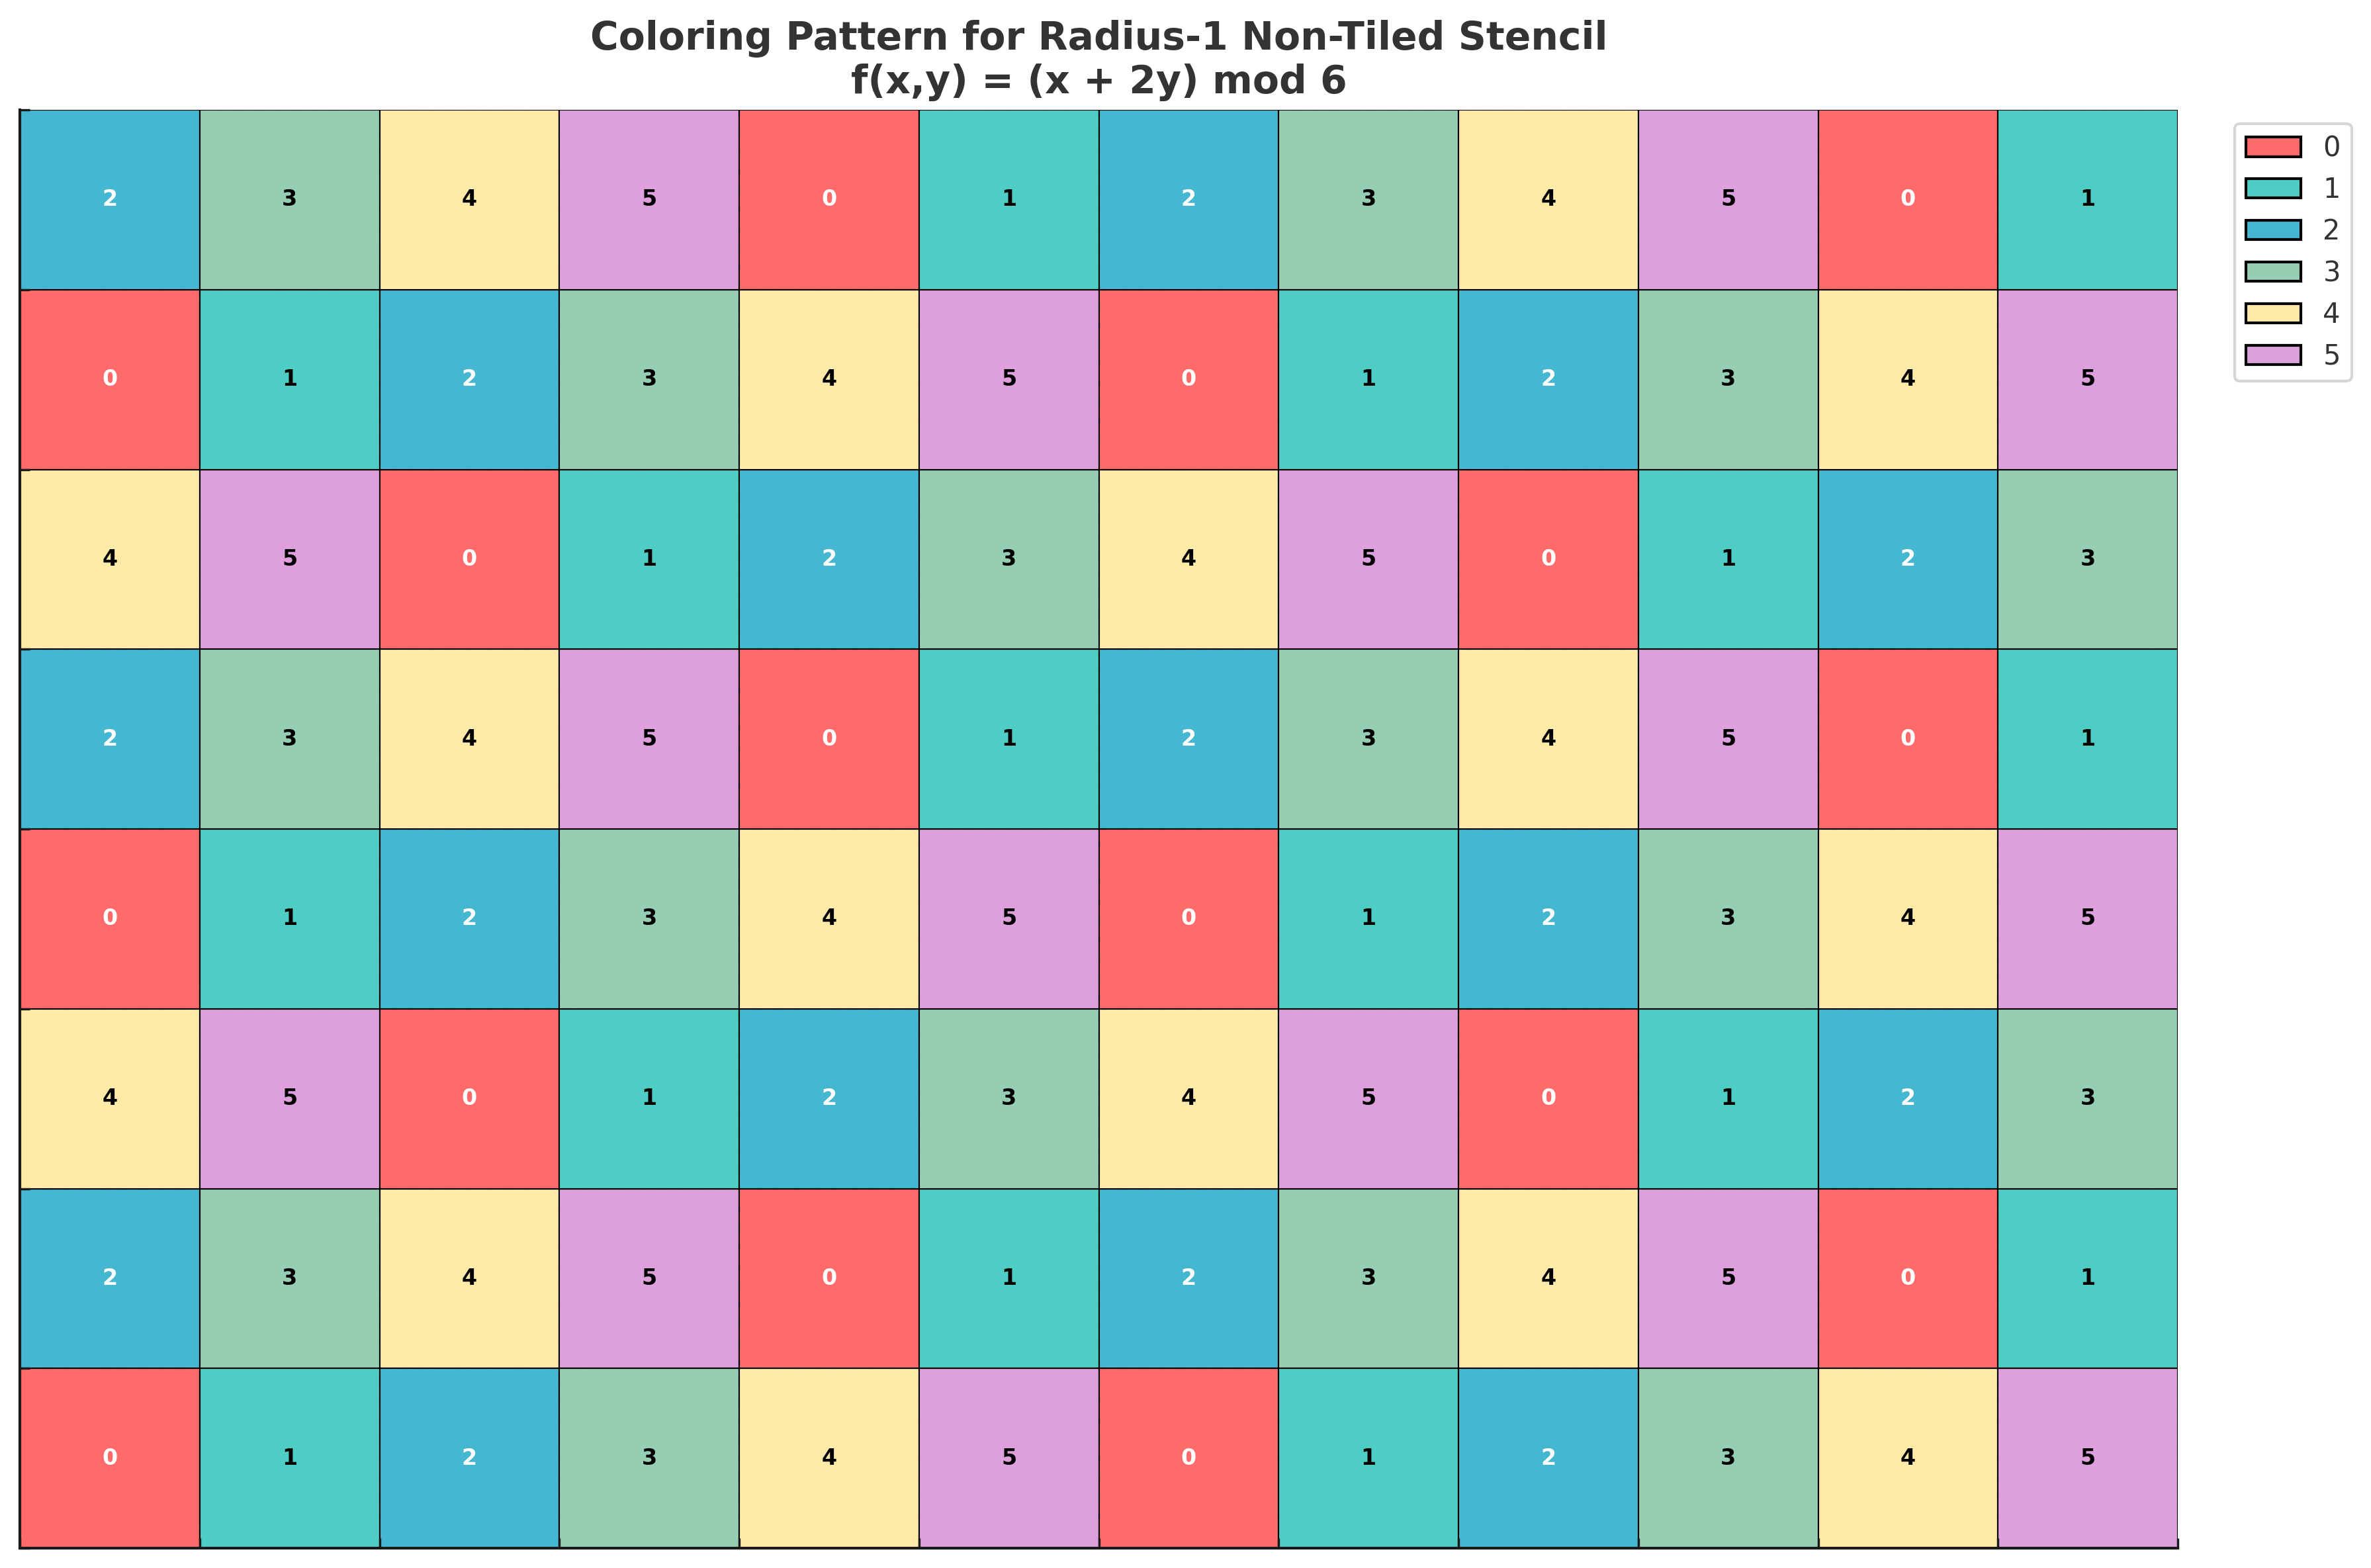
\includegraphics[width=0.5\linewidth]{plots/r1-stencil-coloring.png}
    \caption{Visualization of the coloring pattern for radius-1 non-tiled stencil. Each color represents a distinct routing color (0-5) used for conflict-free communication between PEs. The numbers in each cell show the color index computed by $f(x,y) = (x + 2y) \bmod 6$.}
    \label{fig:r1_stencil_coloring}
\end{figure}
\subsubsection{PE Program}
The implementation for the radius-1, non-tiled case is relatively simple.
Although only single elements are processed at a time, DSDs are needed for communication and for performance reasons explicit DSR assignment is employed, decreasing the number of cycles per iteration significantly.  
Further, the center multiplication is placed at the beginning of each iteration in a way that it overlaps with the communication delay and does not need an additional cycle.
Because only one fp32 element is received from and send to each neighbour, input- and output- queues never fill up completely and synchronous DSD operations can be used instead of asynchronous operations that add significant overhead.
Furthermore, the algorithm multiplies the value which is send to the neighbors with the coefficient $w_1$ while sending, so that the receiving PEs only add these values to $w_0 \cdot v$ to get the new value.
By computing the intermediate values $intermediate_1$ and $intermediate_2$ before adding them to $value$, the number of cycles for this part of the calculation is reduced from 10 to 7.
\begin{algorithm}
    \caption{Algorithm with intermediate values}
    \begin{algorithmic}[1]
        \State $intermediate_1 \gets \Call{ReceiveFromNorth}{} + \Call{ReceiveFromEast}{}$
        \State $intermediate_2 \gets \Call{ReceiveFromSouth}{} + \Call{ReceiveFromWest}{}$
        \State $value \gets value +intermediate_1$
        \State $value \gets value +intermediate_2$
    \end{algorithmic}
\end{algorithm}
While the reason for this performance benefit cannot be explained by the publicly available documentation from Cerebras, speculation from limited testing suggests that values seem to be avilable to a following operation only three cycles after they were written to.
Our empirical analysis revealed a data dependency stall: an operation using a register as an operand is delayed until at least three cycles have passed since that register was last written to. While this behavior is not detailed in the public documentation, it consistently impacts performance. By reordering the computation to use intermediate variables (as shown in Algorithm X), we mitigate these stalls, reducing the cycle count for this computational segment from 10 to 7 cycles.

Unfortunately, this does not work on WSE-3, since it allows at most one fabric DSD arguments per operation.

% table with operation for one grid point
% columns: operation, cerebras op code, count, flops
\begin{table}[h]
    \centering
    \begin{tabular}{|c|c|c|c|}
        \hline
        Operation & Cerebras Op Code & Count & Flops \\
        \hline
        add & \texttt{@fadds} & 4 & 4 \\
        mul & \texttt{@fmuls} & 2 & 2 \\
        \hline
        total & & 6 & 6 \\
        \hline
    \end{tabular}
    \caption{Operations for one grid point and iteration in the radius-1, non-tiled implementation.}
    \label{tab:r1_non_tiled_operations}
\end{table}


\subsection{tiled any radius star shaped 2d}
For a radius greater than one, the computation can be expressed as follows:
\begin{equation}
    \label{eq:stencil_computation_tiled}
    v^{'} = w_0 \cdot v + \sum_{i=1}^{r} w_i \cdot (v_{north,i} + v_{east,i} + v_{south,i} + v_{west,i})
\end{equation}
Where $v$ is the old value of the element, $v_{north,i}, v_{east,i}, v_{south,i}, v_{west,i}$ are the values of the four neighbors at distance $i$ from the center and $w_0, w_1, \dots, w_r$ are the stencil coefficients.
\subsubsection{Routing configuration}
\begin{figure}
    \centering
    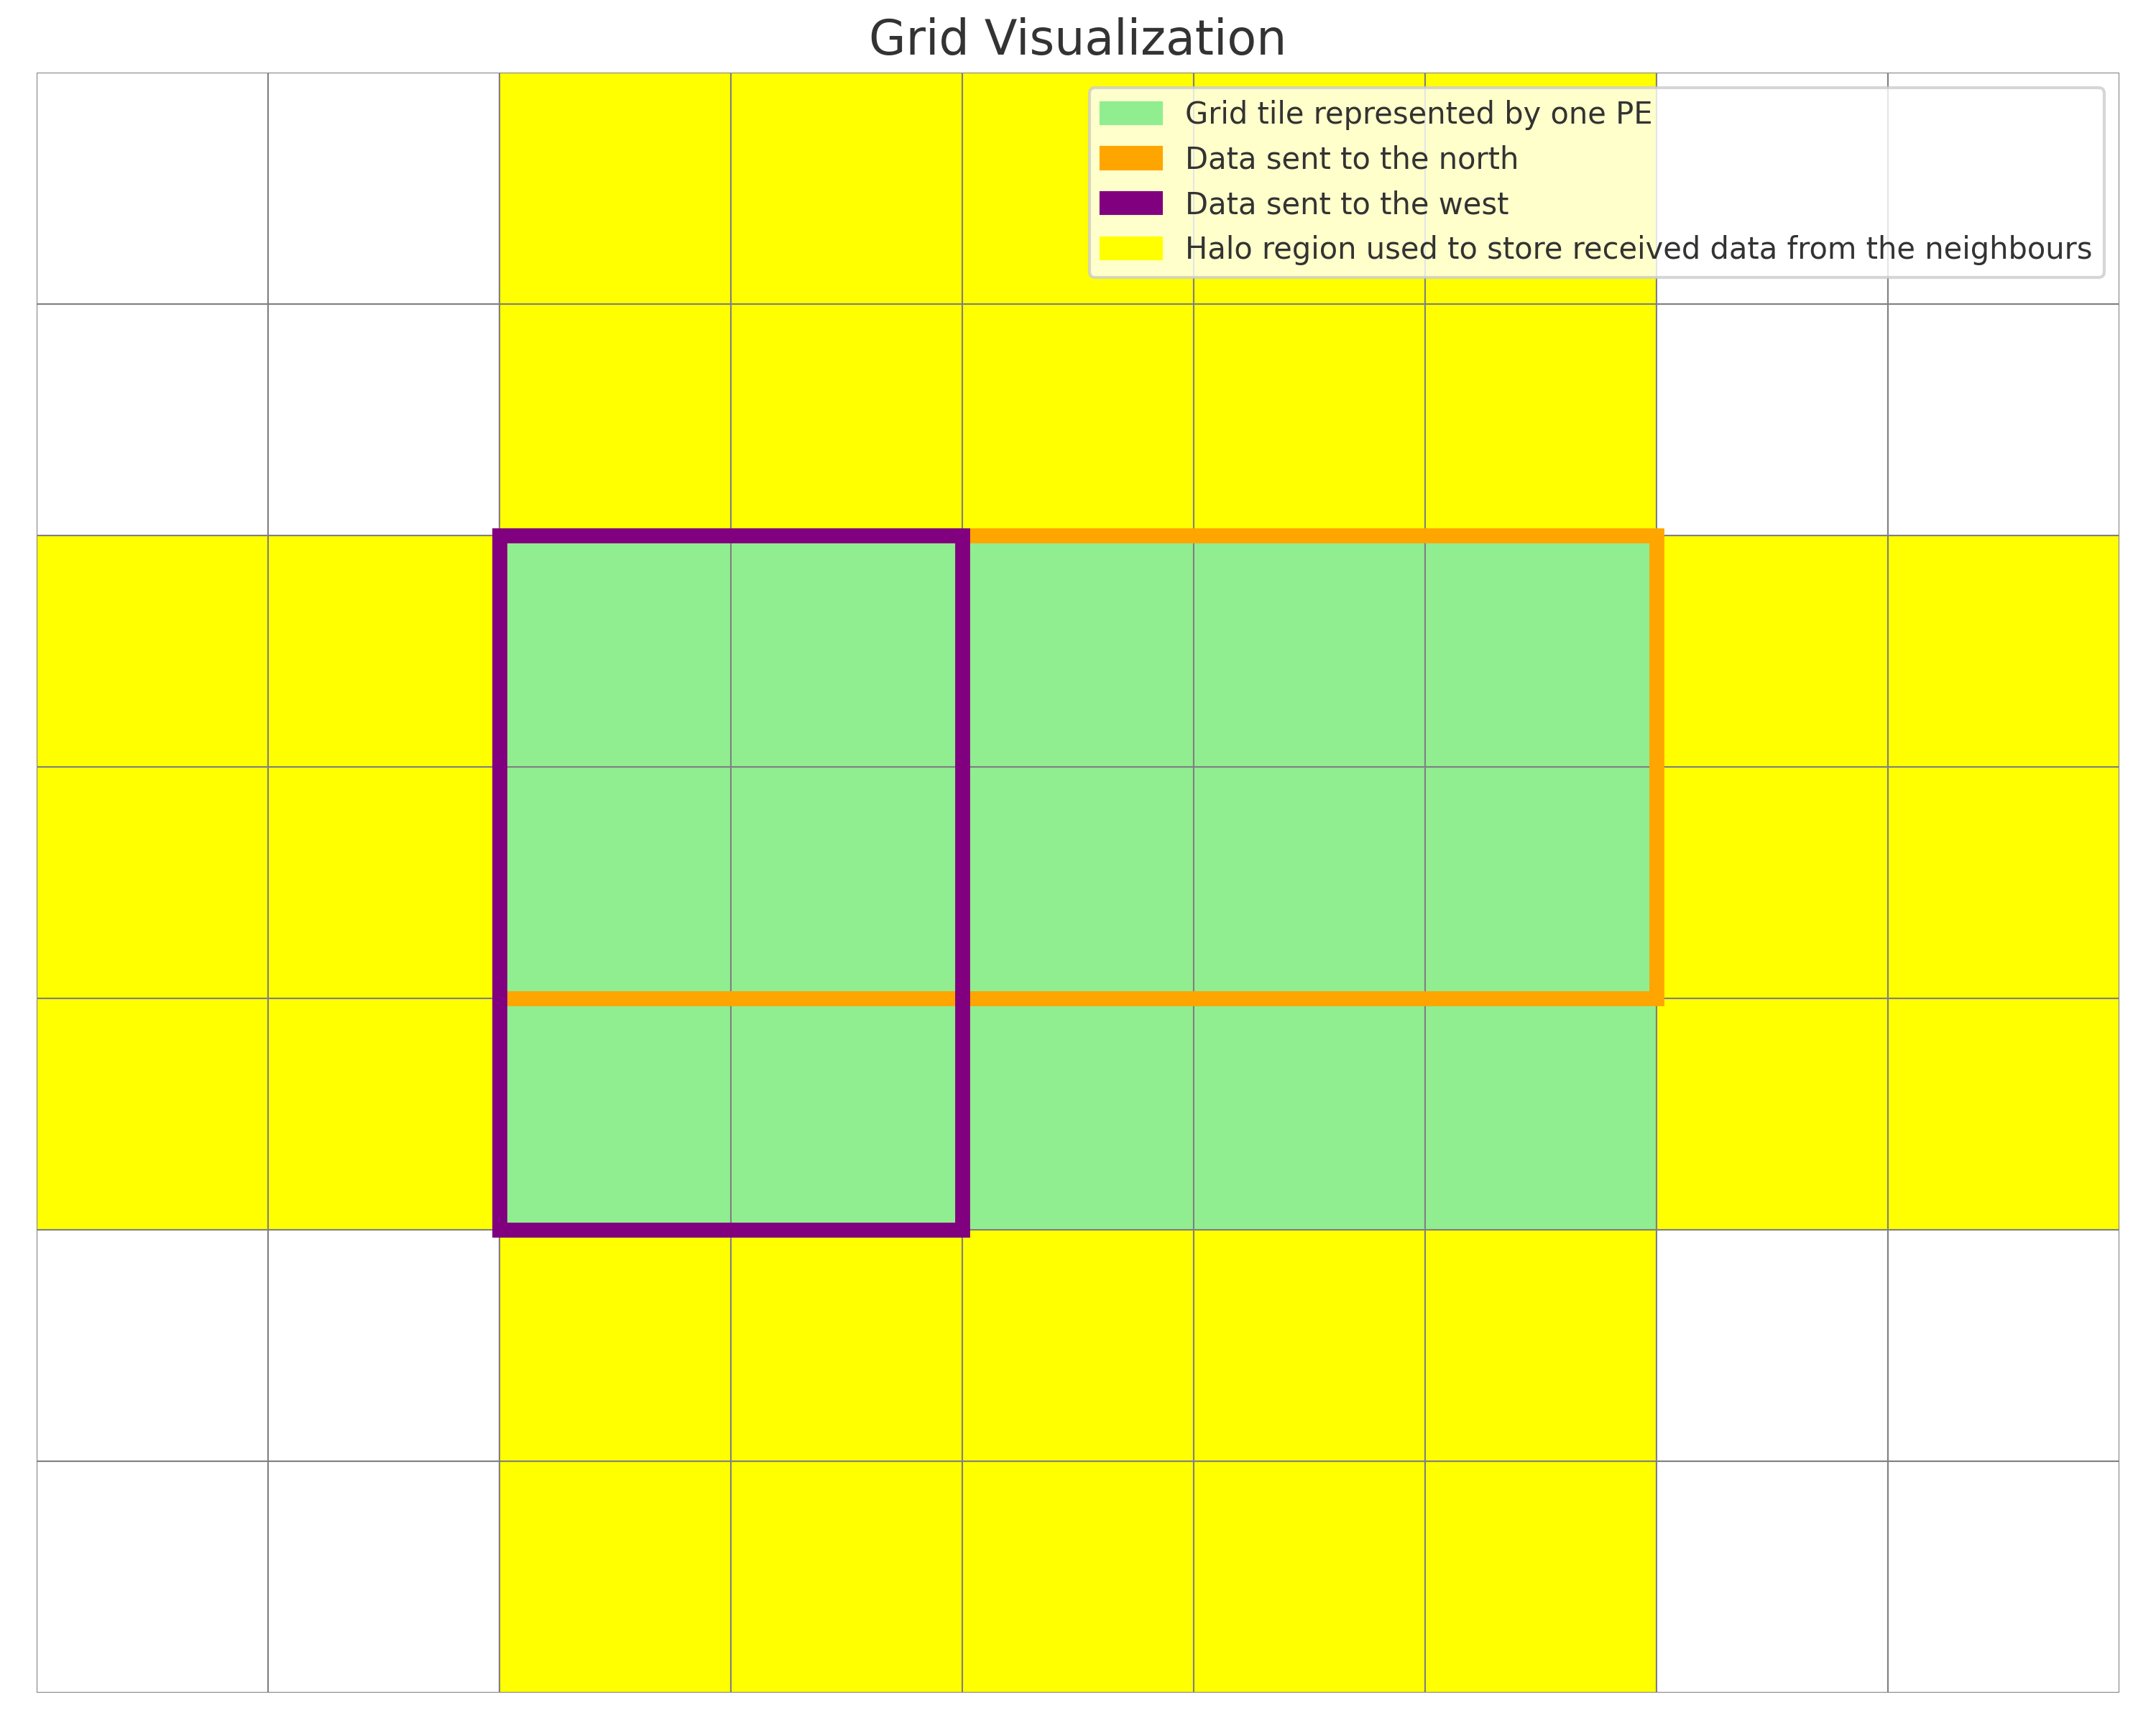
\includegraphics[width=0.5\linewidth]{plots/grid_visualization.png}
    \caption{Visualization of data stored within one PE for tiled stencil. $t_w=5$, $t_h=3$ and $r=2$. The green area is the tile of the grid stored within this PE. The yellow area is what needs to be received from the neighboring PEs in order to compute one iteration. The part surrounded in orange is what needs to be send to the northern PE and and the purple area is what needs to be send to the western PE.}
    \label{fig:grid_visualization}
\end{figure}
The communication for the variable tile size requires one PE to send different data to its neighbors. This is visualized in figure \ref{fig:grid_visualization}. This requires four distinct colors for sending to the different neighbors as well as four colors to receive. For each of the four directions, a pair of colors is used and arranged in a checkerboard pattern across the PE-grid.
If colors 0 and 1 are used for data transfer from west to east, following function can be used to determine what color is used to send and to receive:
\begin{equation}
    \label{eq:tiled_coloring_function}
    f(row, col)=(row+col)\m2
\end{equation}
Where $f$ determines the color used to send data east and $1-f$ is used to receive from west. The same method is also applied for the other directions.
\subsubsection{PE Program}

\begin{figure}
    \centering
    \animategraphics[autoplay,loop,controls=false,width=\linewidth]{0.5}{plots/stencil_frames/frame_0}{0}{8}
    \caption{Visualization of the stencil computation for a radius-2, tiled stencil. (animation might not play in all pdf readers)}
    \label{fig:stencil_algorithm_animation}
\end{figure}

The tile of the grid, held by single PE is stored in the center region of a 2D array of size $(t_h+2r)\times (t_w+2r)$ - the $buffer$. This array is larger than the tile itself to allow for the halo region, which is used to store the data received from the neighbors. Furthermore an accumulator array of the same size is used to store the intermediate values of the stencil computation. In this array, only the center of size $t_h, t_w$ is used. Chosing its size to be the same as the buffer leads to more consistant memory access patterns, which reduces bank conflicts.

Two \texttt{mem4d\_dsd}s per direction are used for communication. One that specifies the location withing in the buffer of the data to send and one that specifies the location of the data to receive.
Asynchronous \texttt{@fmovs} instructions are used for data exchange. Two counters track the completion of asynchronous send and receive operations. Once all four neighbor data blocks have been sent and all four have been received, the main computation task is triggered. This ensures that the computation only starts once all necessary data is available in the halo regions.

A DSD is used to select the center region of the buffer. This DSD is subsequently shifted to represent a rectengual area of the buffer that is shifted up, down, left or right by a number of elements up to the radius from the center. \texttt{@fmacs} instructions are used to multiply these values with the respective weight and add the results to the accumulator. The accumulator is then multiplied with the weight $w_0$ and added to the center region of the buffer to complete the iteration. This process is visualized in figure \ref{fig:stencil_algorithm_animation}.

If only \texttt{@fmacs} instructions were used, the accumulator would have to be reset to zero after each iteration. To avoid this, a \texttt{@fmuls} instruction is used for the very first operation that writes to the accumulator to overwrite the values of the previous iteration \ref{tiled_algorithm_code}.

\begin{algorithm}
    \caption{Tiled algorithm code}
    \begin{algorithmic}[1]
        \State \textbf{for} $i$ from 1 to $r$
        \State \quad if $i==1$
        \State \quad \quad $accumulator \gets weights[i] \cdot buffer\_center\_dsd_{UP,i}$
        \State \quad else
        \State \quad \quad $accumulator \gets accumulator + weights[i] \cdot buffer\_center\_dsd_{UP,i}$
        \State \quad $accumulator \gets accumulator + weights[i] \cdot buffer\_center\_dsd_{DOWN,i}$
        \State \quad $accumulator \gets accumulator + weights[i] \cdot buffer\_center\_dsd_{LEFT,i}$
        \State \quad $accumulator \gets accumulator + weights[i] \cdot buffer\_center\_dsd_{RIGHT,i}$
        \State \textbf{end for}
        \State \quad $buffer_center_dsd \gets buffer_center_dsd + weights[0] \cdot accumulator$
    \end{algorithmic}
\end{algorithm}

The dicrilet border is implemented by using a ring of PEs that only send and receive data from their neighbors and do not participate in the computation. If $r<t_w$ or $r<t_h$ the border PEs values are padded with zeros to fill their buffer.

\begin{table}[h]
    \centering
    \begin{tabular}{|c|c|c|c|}
        \hline
        Operation & Cerebras Op Code & Count & Flops \\
        \hline
        fmac & \texttt{@fmacs} & 5r-1 & 10r-2 \\
        mul & \texttt{@fmuls} & 1 & 1 \\
        \hline
        total & & 5r & 10r-1 \\
        \hline
    \end{tabular}
    \caption{Operations for one grid point and iteration, tiled implementation with radius $r$.}
    \label{tab:tiled_operations}
\end{table}


As a special case of the tiled algorithm, the radius-1 problem was further optimized by using \texttt{mem1d\_dsd}s instead of \texttt{mem4d\_dsd}s for the halo regions where the neighbors data is received as well as the data to send. Furthermore the shifted DSDs are precomputed and all DSDs are explicitly assigned to distinct DSRs. There are enough DSRs available so that each DSR is used for at most one DSD. This allows for a significant reduction in the number of cycles per iteration, since loading the DSDs into DSRs only needs to be done once, independent of the number of iterations. We still find that the DSDs used for reading the parts of the buffer that are send to the neighbors and the onces describing the halo regions for receiving need to be reloaded to the DSRs for each iteration. The load to DSR for these DSDs acts as a kind of reset and if not done, it leads to buffer overflows. The documentation doesn't specify this requirement and interestingly, it is not necessary for all DSDs. 
As another optimization, \texttt{@fadds} are used instead of \texttt{@fmacs} and the multiplication is handled separately. This reduces the flop number from $9$ to $6$ per element and results in a perfomance improvement because the simd width for \texttt{@fadds} is 2/4 on wse-2/3 while it is only 1 for \texttt{@fmacs} \ref{tiled_algorithm_code_r1}. Note that the shifted DSDs$buffer\_center\_dsd_{DIR,i}$ in the general version need to be created for each iteration of the loop while pre-computed DSDs are used in this optimized version.

We refer to this as the r1 optimized version of the tiled algorithm.
The tiled algorithm is implemented so that it automatically selects the r1 optimized version if the radius is 1.
For all experiments in this work, the r1 optimized version is used whenever applicable, except when explicitly stated otherwise.

\begin{algorithm}
    \caption{Radius-1, tiled algorithm code}
    \begin{algorithmic}[1]
        \State $accumulator \gets buffer\_center\_dsd \cdot weights[0]/weights[1]$
        \State $accumulator \gets accumulator + buffer\_center\_dsd_{UP,1}$
        \State $accumulator \gets accumulator + buffer\_center\_dsd_{DOWN,1}$
        \State $accumulator \gets accumulator + buffer\_center\_dsd_{LEFT,1}$
        \State $accumulator \gets accumulator + buffer\_center\_dsd_{RIGHT,1}$
        \State $buffer\_center\_dsd \gets buffer\_center\_dsd + accumulator \cdot weights[1]$
    \end{algorithmic}
\end{algorithm}

\begin{table}[h]
    \centering
    \begin{tabular}{|c|c|c|c|}
        \hline
        Operation & Cerebras Op Code & Count & Flops \\
        \hline
        add & \texttt{@fadds} & 4 & 4 \\
        mul & \texttt{@fmuls} & 2 & 2 \\
        \hline
        total & & 6 & 6 \\
        \hline
    \end{tabular}
    \caption{Operations for one grid point and iteration, r1 optimized tiled implementation.}
    \label{tab:tiled_operations_r1_optimized}
\end{table}

With a larger tile size, the explicit starting mechanism of the computation task can be skipped so that the computation task can be activated while the data is send and received. Explicitly specified task priorities lead to the computation task only being executed after all data is send and received. However, this only works for WSE-3.

\section{Theretical performance evaluation and comparison against roofline model....}
actual roofline plot
\subsection{Radius 1, no tiling}
In this section the theoretical best performance of the implemented algorithms given the Cerebras hardware constraints is analyzed.
We assume the data type to be float32.
The cycle count for one iteration of the stencil is limited by following factors:
\begin{itemize}
    \item Communication time, i.e. total amount of data send and received per iteration divided by link throughput
    \item Computation time, i.e. total amount of computation per iteration divided by computation throughput
    \item Communication delay, i.e. total amount of time spent waiting for data while no computation can be done
\end{itemize}
The CE must receive the values from its four neighbors. Since the link capacity between the router and CE is 32 bit per cycle, this will take four cycles in the best case.

The received data can immediately be used for computation as the \texttt{@fadds} and \texttt{@fmacs} commands can use dsds of type \texttt{fabin\_dsd} as an input. This means most of the computation can be done during the receiving of the data. Only one extra cycle is necessary to take into account the old $value$. With a clever implementation this extra computation could be executed during the communication delay idle time so that it doesn't affect the overall cycle count.

Sending takes one cycle from CE to its router, another cycle from the router to its neighbors routers and a third cycle from these routers to the neighbors CEs. This results in three cycles for the communication delay.

In total this results in seven cycles per stencil operation that could be archived in theory.
Note that this is independent of the actual grid size (as long as it fits onto the WSE).


\subsection{Any radius and tiling}
Similarly to before the total computation for one iteration can be split up into the same three fundamental steps. We now need to take the radius $r$, tile width $t_w$ and tile height $t_h$ into account.

Each PE needs data from its four neighbors. $r\cdot t_w$ elements from the northern and southern neighbors and $r\cdot t_h$ elements from the western and eastern neighbors. This results in $2r(t_w+t_h)$ total elements and cycles for data receiving.

During the computation $4r+1$ multiply-add operations per grid element are required which results in $t_wt_h(4r+1)$ multiply-add operations per PE. With SIMD execution we can parallelize this and divide it by the SIMD width for \texttt{@famcs} which is 4 on wse-2 and 8 on wse-3. This results in $\left\lceil\frac{t_wt_h(4r+1)}{s}\right\rceil$. This term exceeds the communication term for most parameter combinations of $t_w,\ t_h$ and $r$. Assuming the first part of the computation could still be done during communication, we can drop the communication term completely. Note that this is a rather optimistic assumption and likely not achievable with the hardware.

The communication delay is in this case negligible and could be overlapped with the computation in a way that it doesn't affect the cycle count. 

This results in a total cycle count of $\left\lceil\frac{t_wt_h(4r+1)}{s}\right\rceil$ which is just the computation time and assuming we can fully overlap the communication time as an optimistic estimate. As a slightly pessimistic estimate we get $\left\lceil\frac{t_wt_h(4r+1)}{s}\right\rceil+2r(t_w+t_h)$ which assumes no possible overlap between communication and computation. 

It becomes clear that for radius 1 the tiled stencil gets significantly slower than the non-tiled implementation. 
\begin{figure}
    \centering
    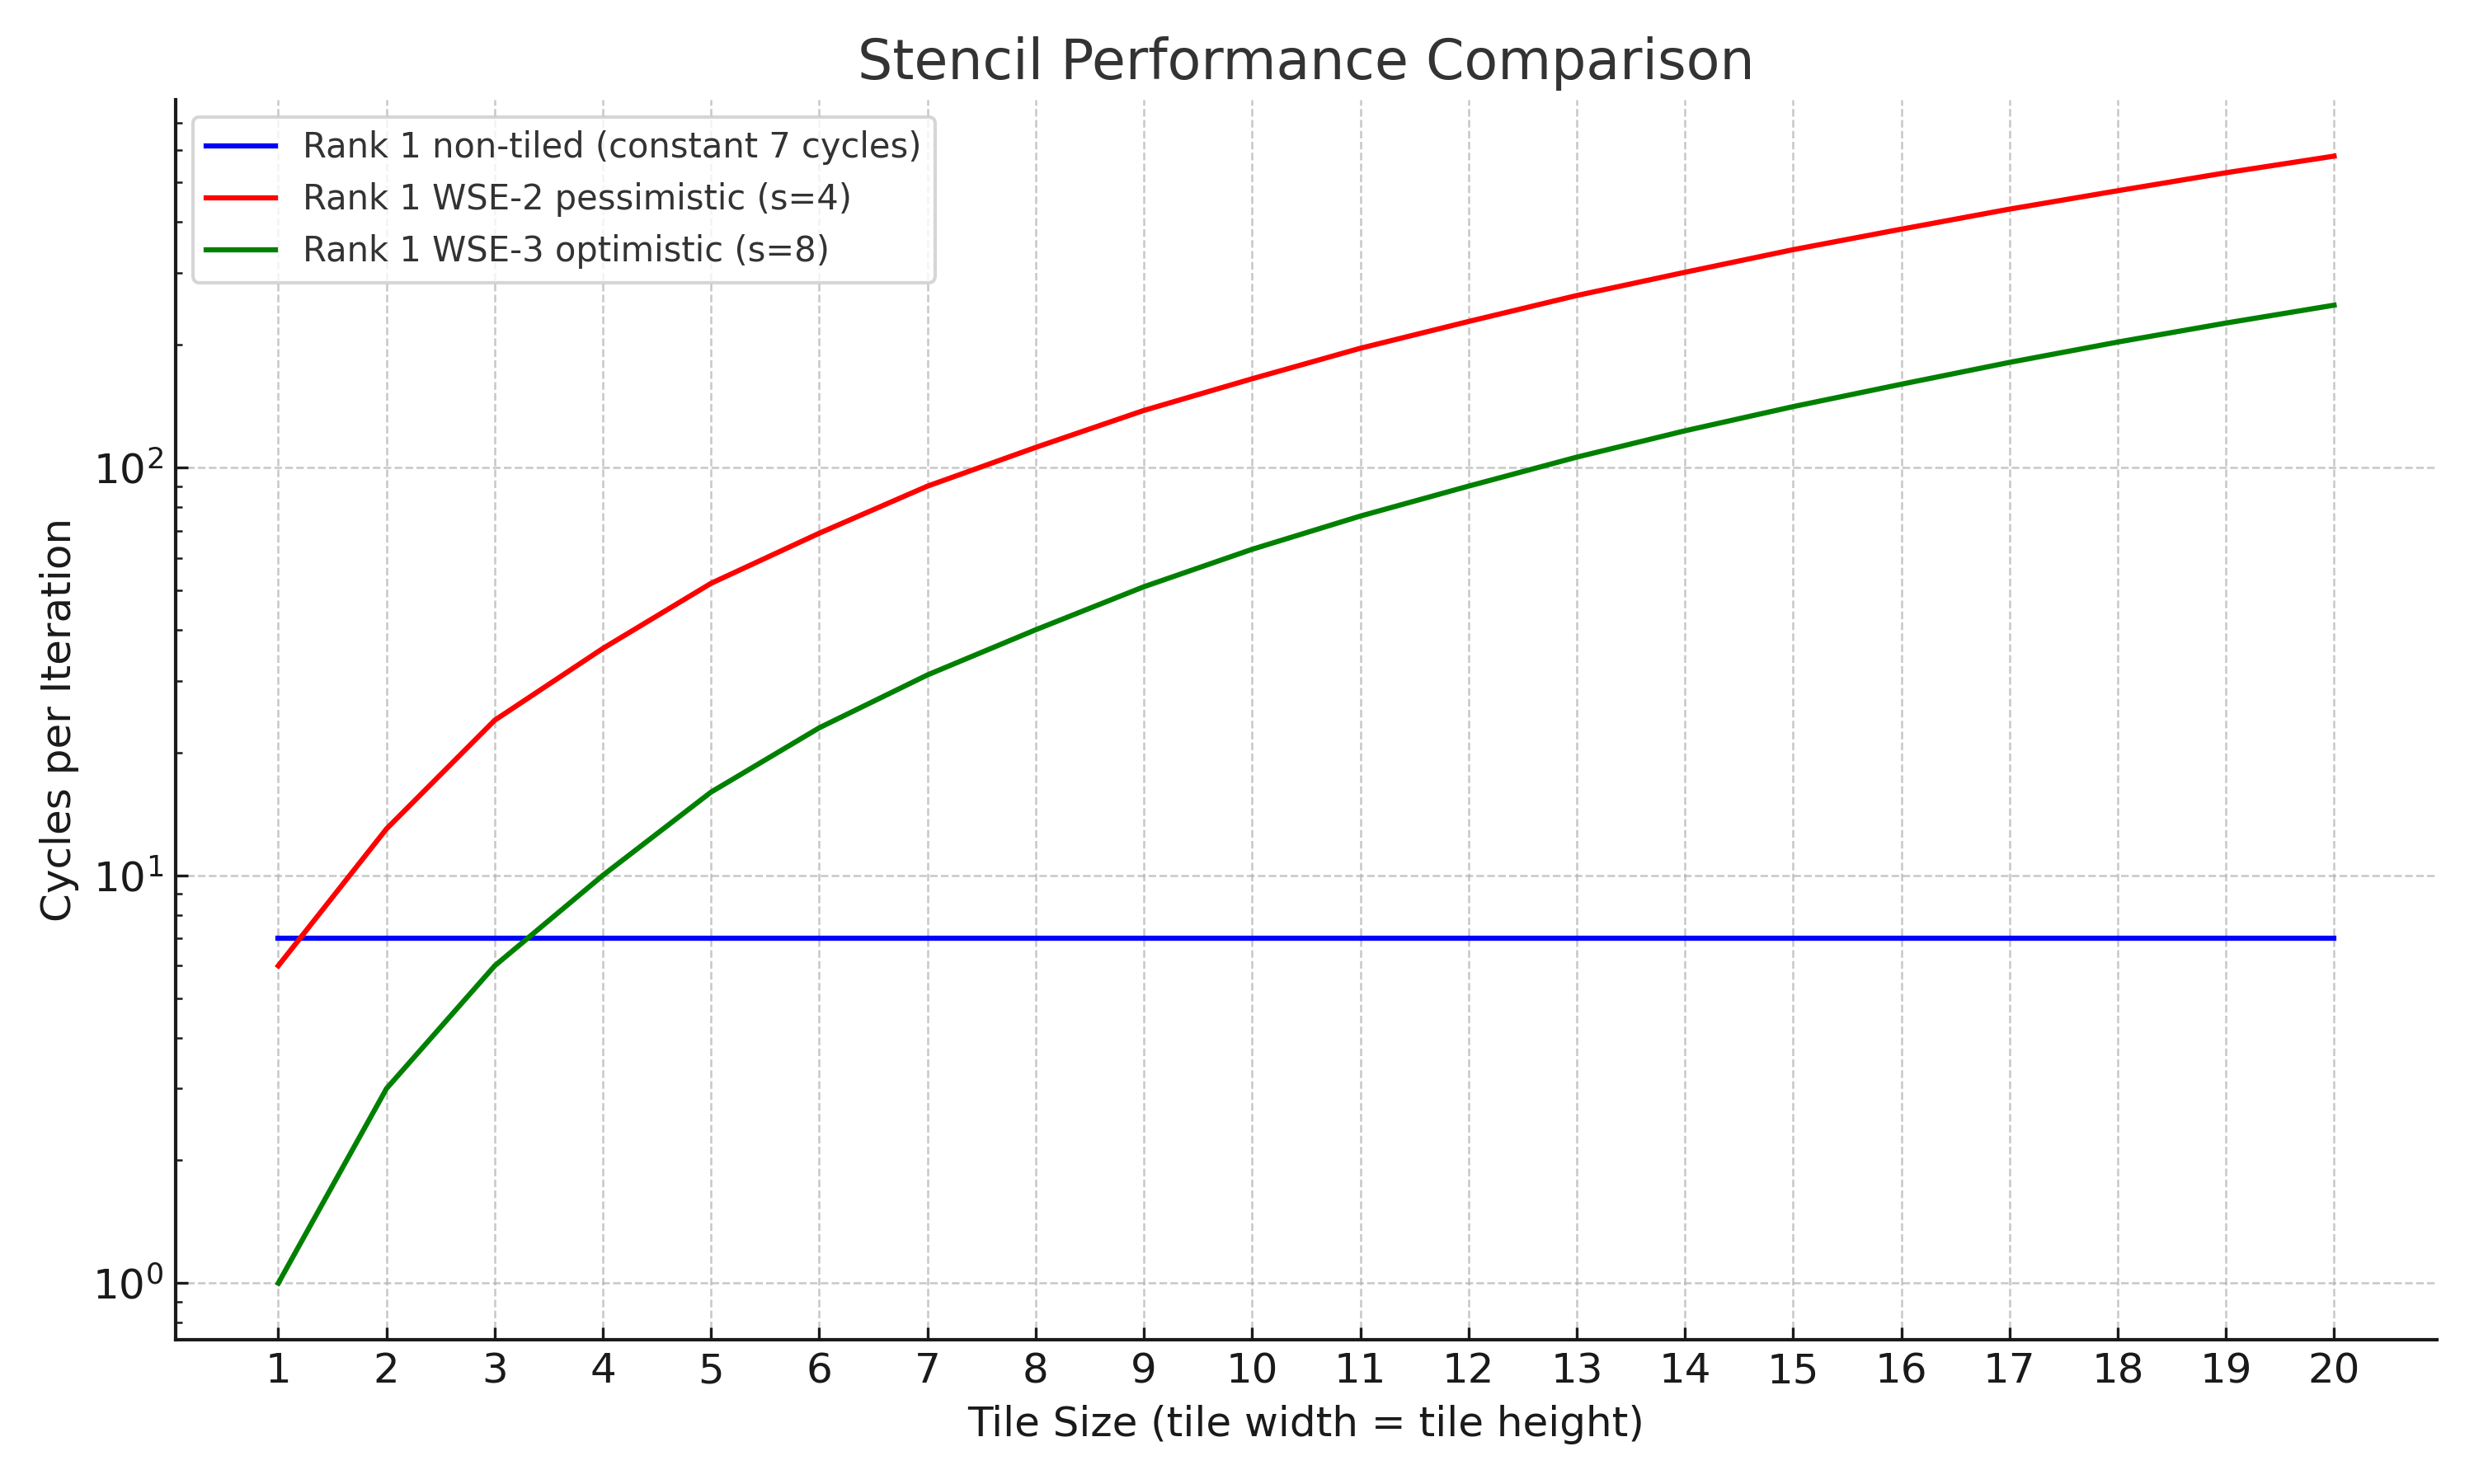
\includegraphics[width=0.5\linewidth]{plots/stencil_performance_comparison.png}
    \caption{Cycles per iteration for tiled and non-tiled stencils theoretical performance with radius 1 }
    \label{fig:enter-label}
\end{figure}



\section{Experiments}
We did several experiments to answer the following questions:
\begin{enumerate}
    \item How stable is the cycle count per iteration?
    \item Is there any overhead for more PEs?
    \item When using a fixed grid size, how does the performance of using more PEs compare to using larger tiles on fewer PEs?
    \item What is the maximum tiling size that fits into the memory of a PE?
    \item How does the performance of the generalized algorithm compare to the specialized algorithm for radius 1?
    \item How does the Cerebras implementation compare to highly optimized implementations on traditional HPC-Arcitectures (CPU, GPU)?
    \item (How does a 2d stencil compare to a 3d stencil?)
    \item What contributes to the cycle count?
    \item How does the r1-optimized tiled algorithm for compare to the non-optimized tiled algorithm
\end{enumerate}

All experiments are performed on the cycle accurate simulator that is part of the Cerebras SDK.
Using the simulator limits the number of PEs and number of iterations so that the data needs to be extrapolated to the whole grid.
We examine to what extend extrapolation is possible in the first two experiments.

We count the cycles used per iteration in the simulator and use this together with the clock speed of the WSE to calculate the time per iteration.

One difference between the simulator and the real hardware is that the simulator does use a single clock for all cores, while the real hardware has a separate clock for each core. (verify this!!!) Because these clocks are not perfectly synchronized, especially experiments with a large number of PEs could differ in the cycle count. Although this is not guaranteed for our algorithm, (source) find that in practice the slighly desynchronized clocks improve overall performance compared to the simulator. 

\subsection{Stability of cycle count per iteration}
For this experiment, we fix the grid size, tile size and radius and run the simulation for different number of iterations.
After two iterations of varying cycle count, the cycle is mostly stable.
For a grid size of 10x10, the cycle count per iteration is $16\pm1$ on WSE-2 and $23\pm1$ on WSE-3.

For a grid of 10x10, and a tile size of 1x1 and radius 1, the tiled algorithm achives $127\pm0$ cycles per iteration on WSE-2 and $156\pm1$ cycles per iteration on WSE-3.

A larger problem size with a grid of 100x100, tile size of 10x10 and radius 5, results in a cycle count per iteration of $3353\pm20$ on WSE-2 and $3377\pm5$ on WSE-3.

Because of the high flucuations in the cycle count in the first two iterations, we measure the cycle count in the following experiments as an average of the 3rd and 4th iteration.

\begin{figure}[h]
    \centering
    \begin{subfigure}[b]{0.48\textwidth}
        \centering
        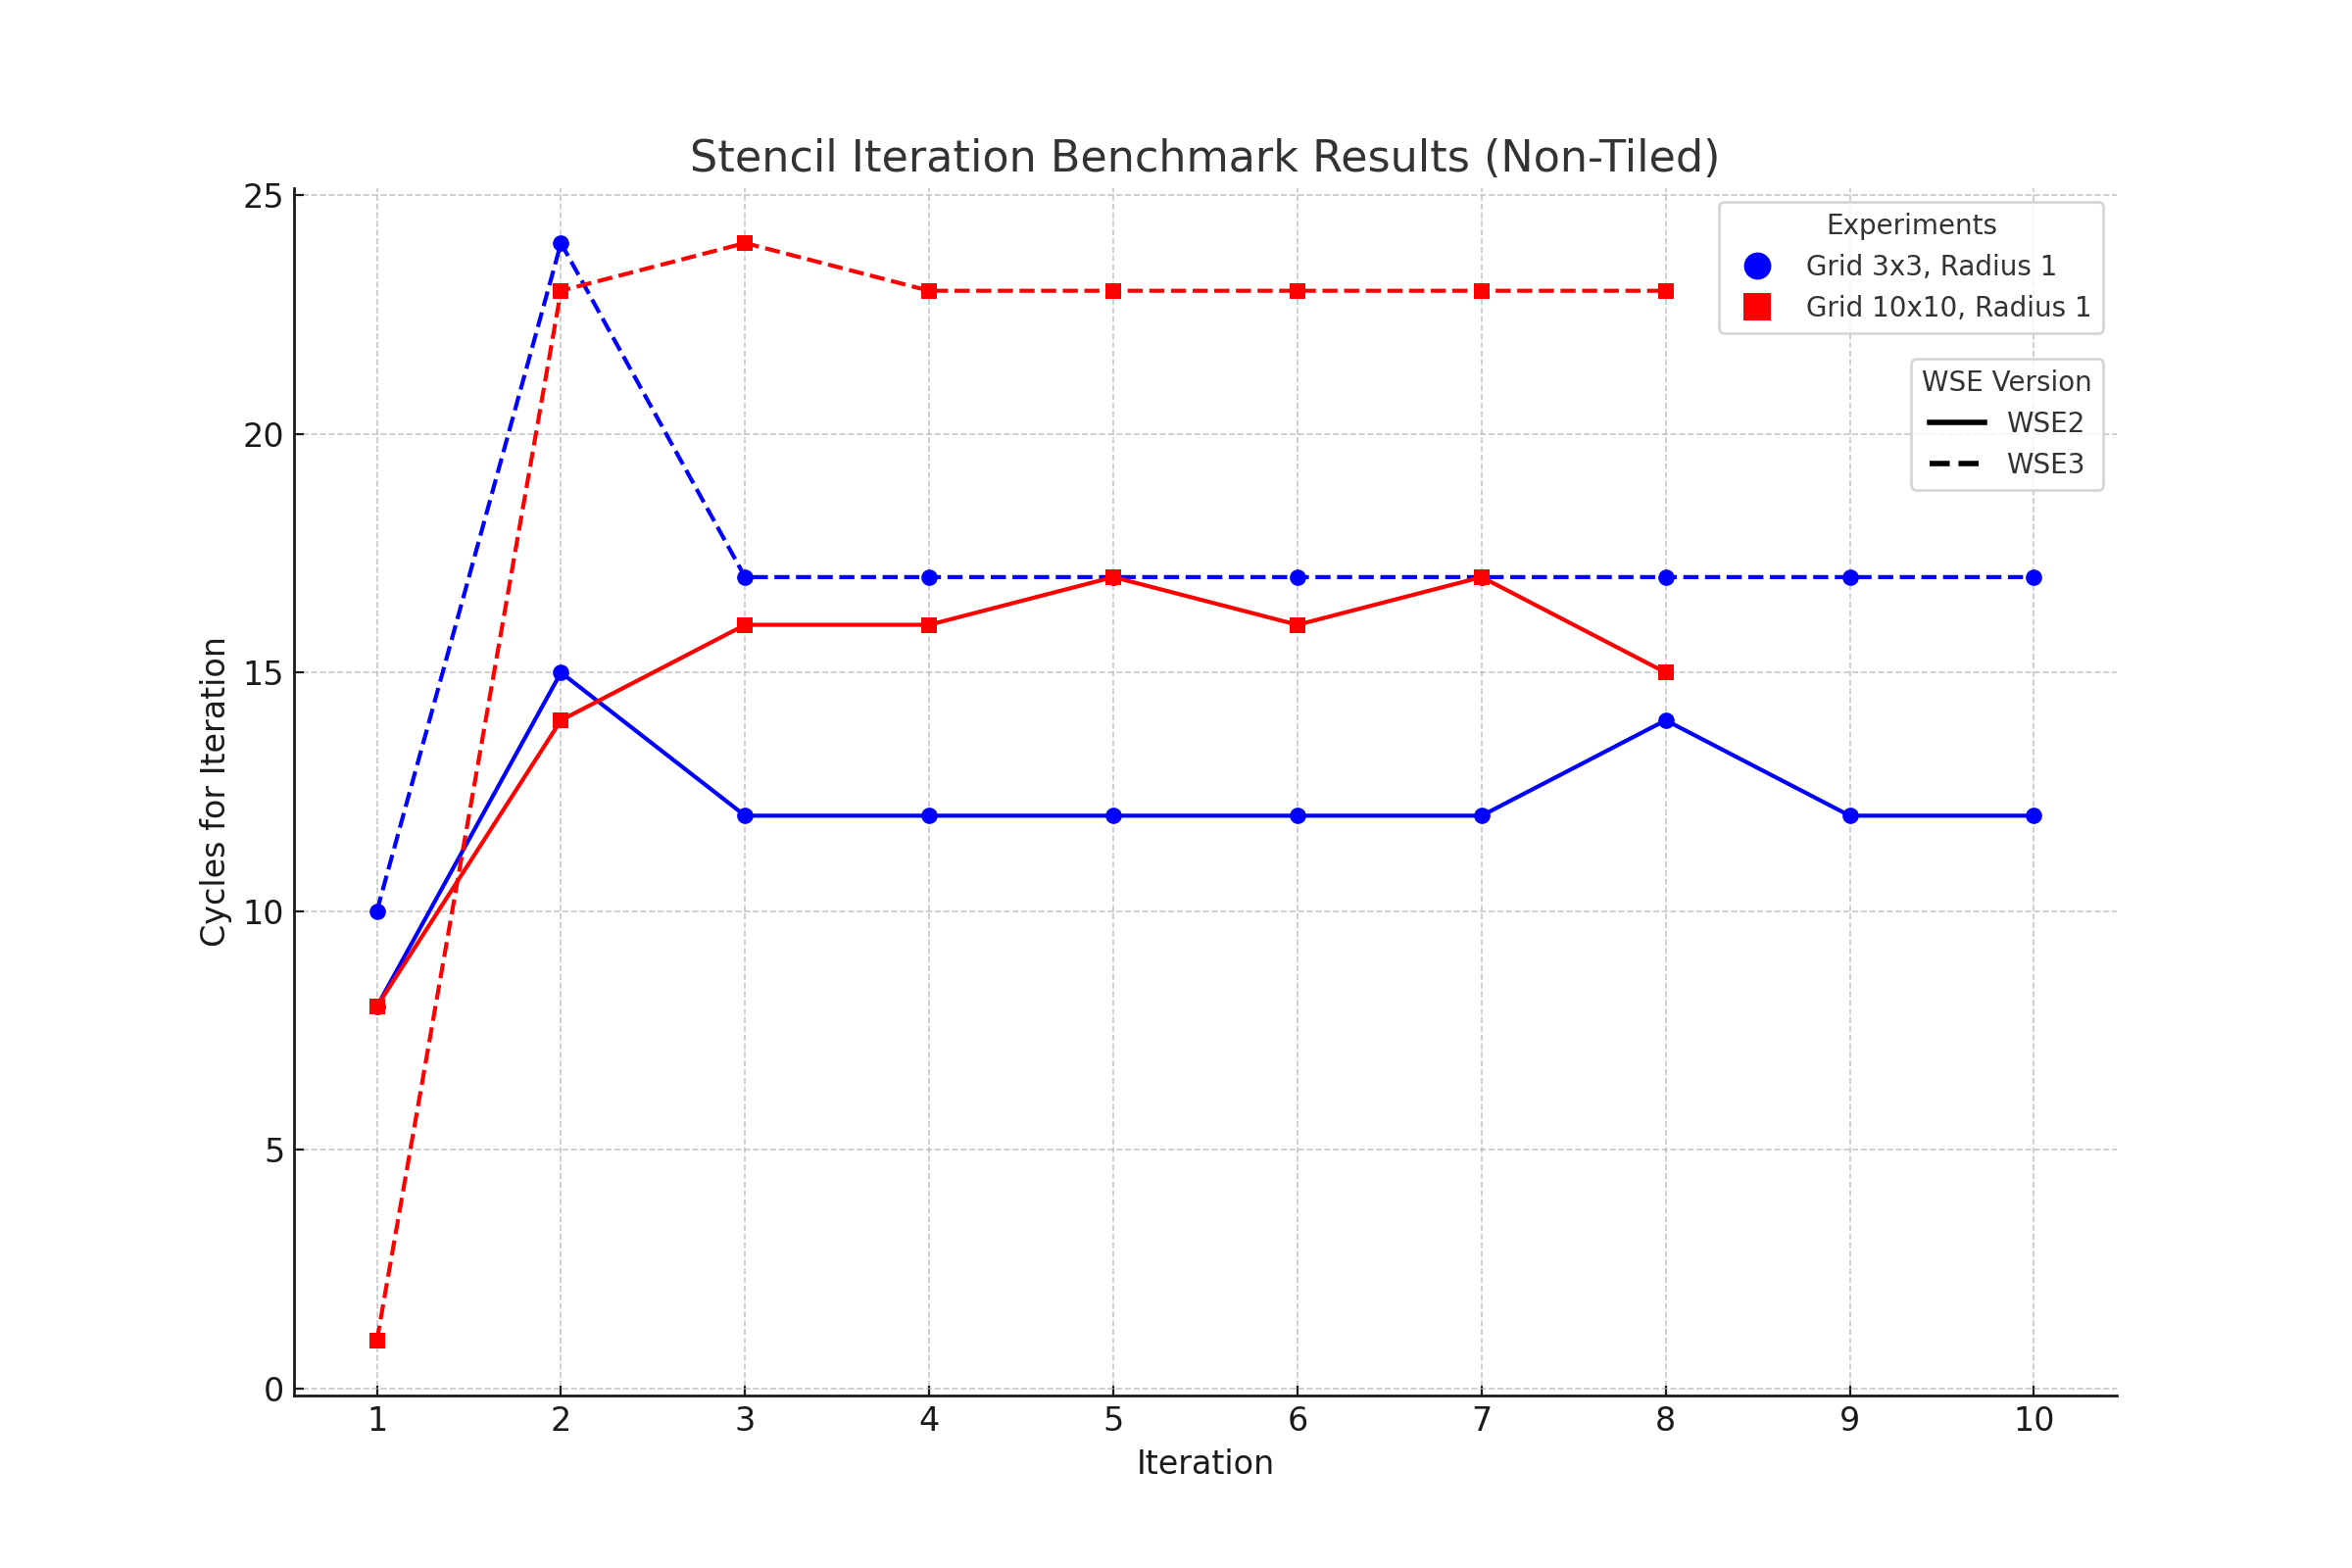
\includegraphics[width=\textwidth]{plots/non_tiled_iteration_stability.png}
        \caption{Non-tiled algorithm}
        \label{fig:non_tiled_iteration_stability}
    \end{subfigure}
    \begin{subfigure}[b]{0.48\textwidth}
        \centering
        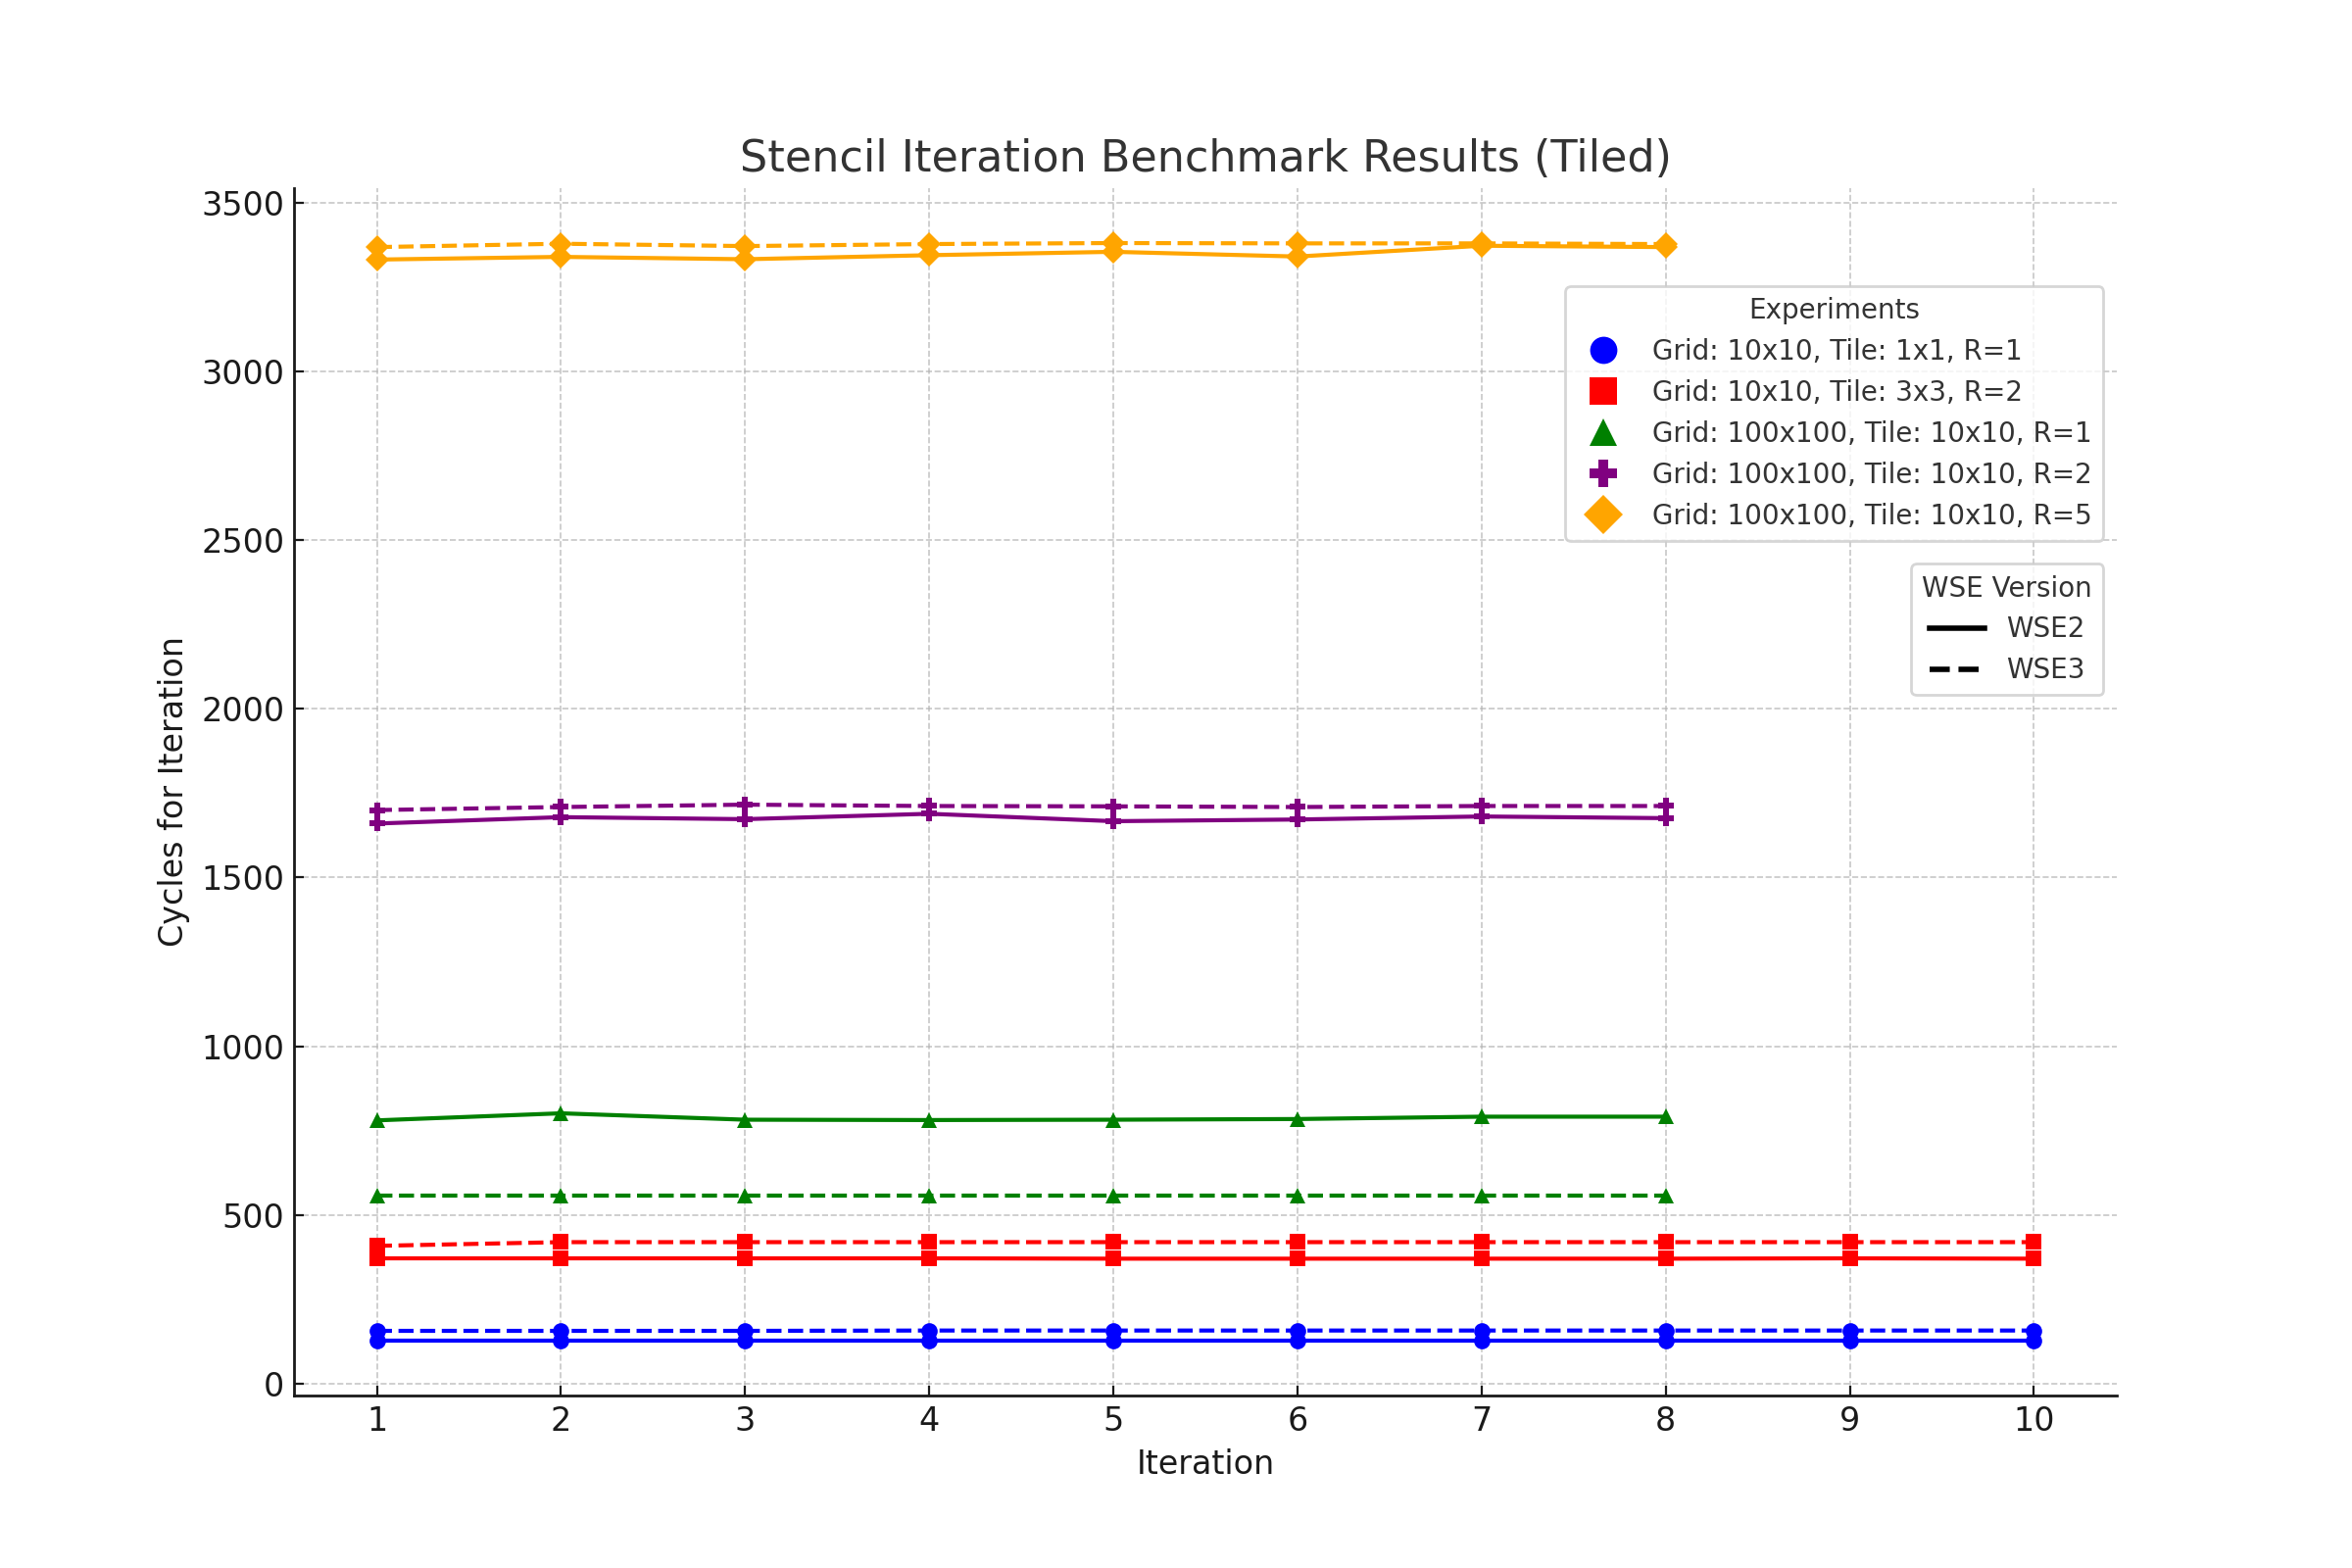
\includegraphics[width=\textwidth]{plots/tiled_iteration_stability.png}
        \caption{Tiled algorithm}
        \label{fig:tiled_iteration_stability}
    \end{subfigure}
    \caption{Cycle count per iteration for non-tiled and tiled algorithm}
    \label{fig:iteration_stability}
\end{figure}


\subsection{Overhead for more PEs}
A very interesting question is how the performance scales with the number of PEs.
As each PE is independent from the others, the time per iteration should be independent from the number of PEs.
This can be confirmed by the tests on the simulator up to a PE count of 400 (20x20).
For a very small number of PEs, the cycle count is slightly faster, but is constant for larger numbers of PEs.

\begin{figure}[h]
    \centering
    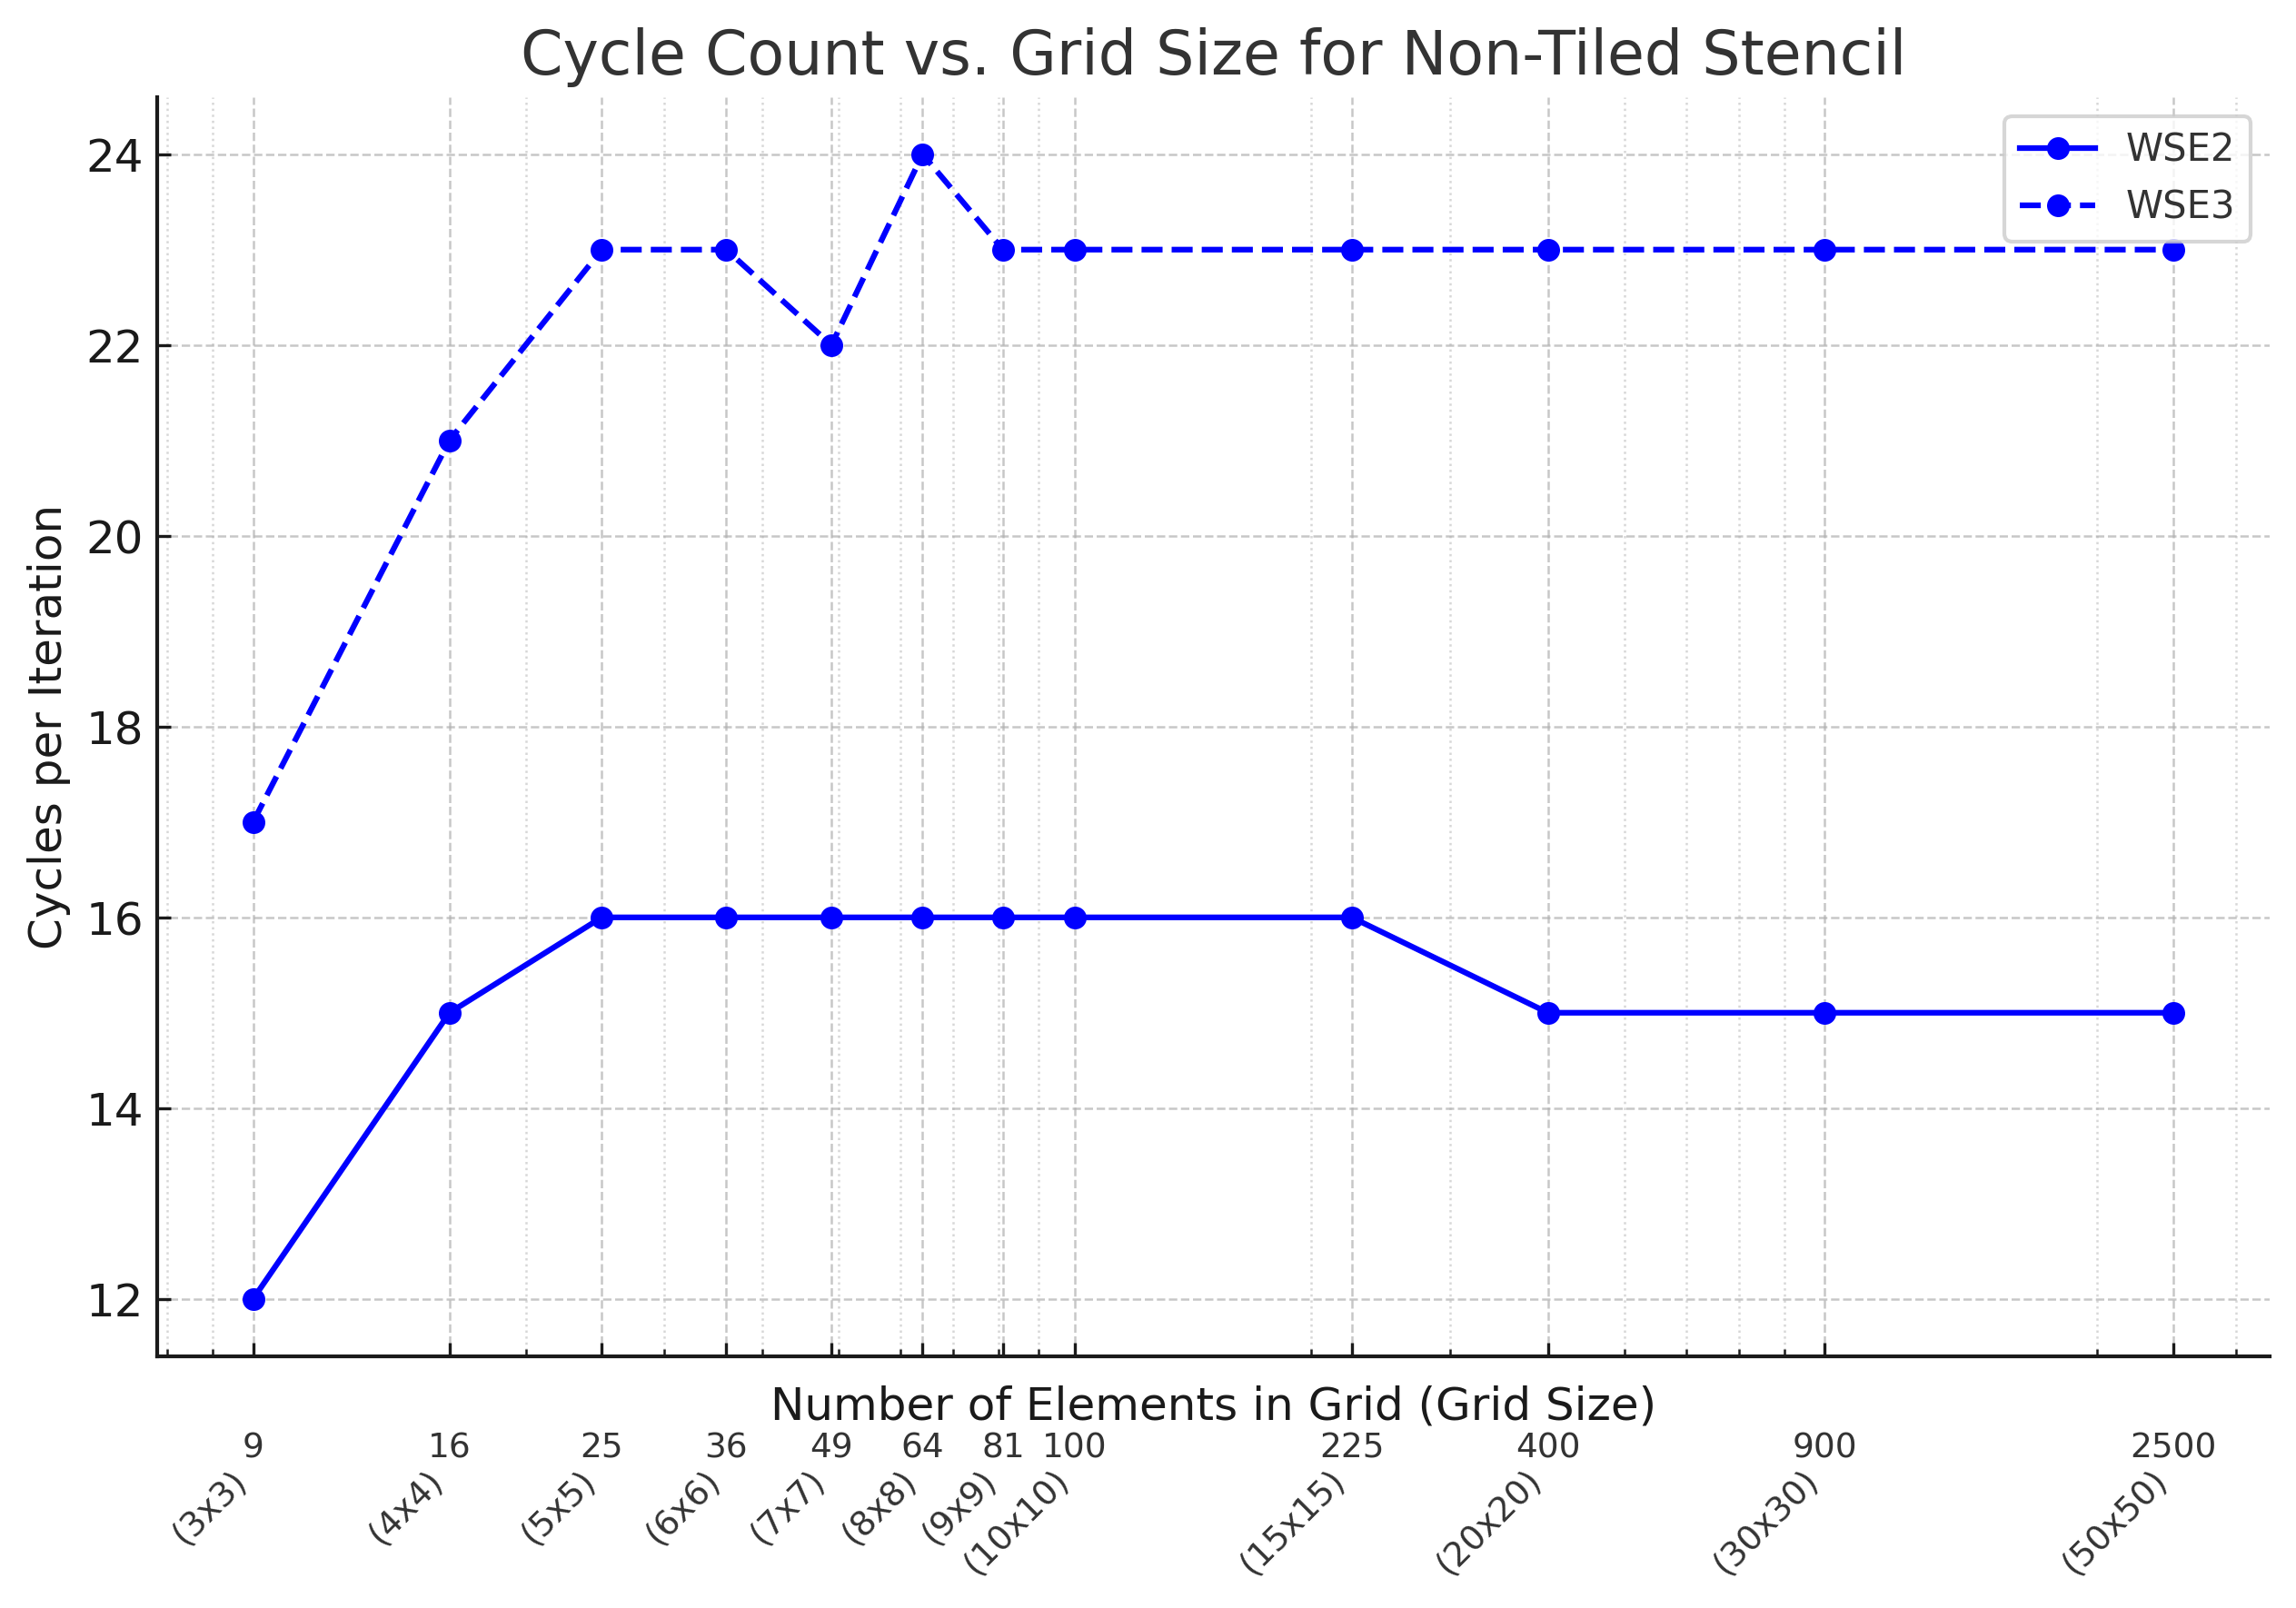
\includegraphics[width=0.5\linewidth]{plots/pe_overhead_non_tiled.png}
    \caption{Cycle count per iteration for different grid sizes for the non-tiled stencil. For very small grid sizes, the cycle count is lower. For larger grid sizes, the cycle count is constant.}
    \label{fig:pe_overhead}
\end{figure}

(citation here) shows that for a 3d stencil that is tested on real hardware.

We therefore expect that our implementation also scales perfectly (or nearly perfectly) on the real hardware.

A possible explanation for significantly faster iterations on the non-tiled stencil in the case of a 3x3 grid size is as follows. Since only the center PE is computing and all other 8 PEs are border PEs do communication only, the center PE doesn't have to wait to receive the data from its neighbors, but can start the next iteration as soon as the previous iteration finishes.

So there is no communication-delay as explained in section \ref{sec:theoretical_performance_evaluation_and_comparison_against_roofline_model}.

For the following experiments we set the parameters so that there are always at least 3x3 PEs that do computation. In this case, the center PE has to wait for all four neighbors that also do real computation.

\subsection{Maximum tiling size}
The maximum tiling size that fits into the memory of a PE is limited by the number of memory banks and the size of the data structure registers.
We test this by increasing the tile size to the maximum that still compiles for (test wse2 and wse3 independently!!! currently same number for both (smaller one))

We find that the maximum tiling size  is 64x64=4096 elements.
A non-quadratical tile size, that results in 4096 elements, is likely also possible, but not tested.
Tile size of 64x64 was tested up to radius 3. It is likely to decrease for larger radius.

This results in a maximum grid size of 48000x51000 on wse-2 and 48000x76000 on wse-3. (calculate correct number here!!!)

\subsection{Comparison of non-tiled and tiled algorithm}

The non-tiled algorithm is implemented in a completely different way than the tiled algorithm.
This allows for a very optimized implementation, that doesn't require any runtime DSD to DSR transfers, asynchronous operations and task activation.
It is therefore significantly faster than the tiled algorithm for radius 1.
However, the non-tiled algorithm is naturally limited to a radius of 1 and a grid size not larger than the WSE dimensions.

\begin{figure}[h]
    \centering
    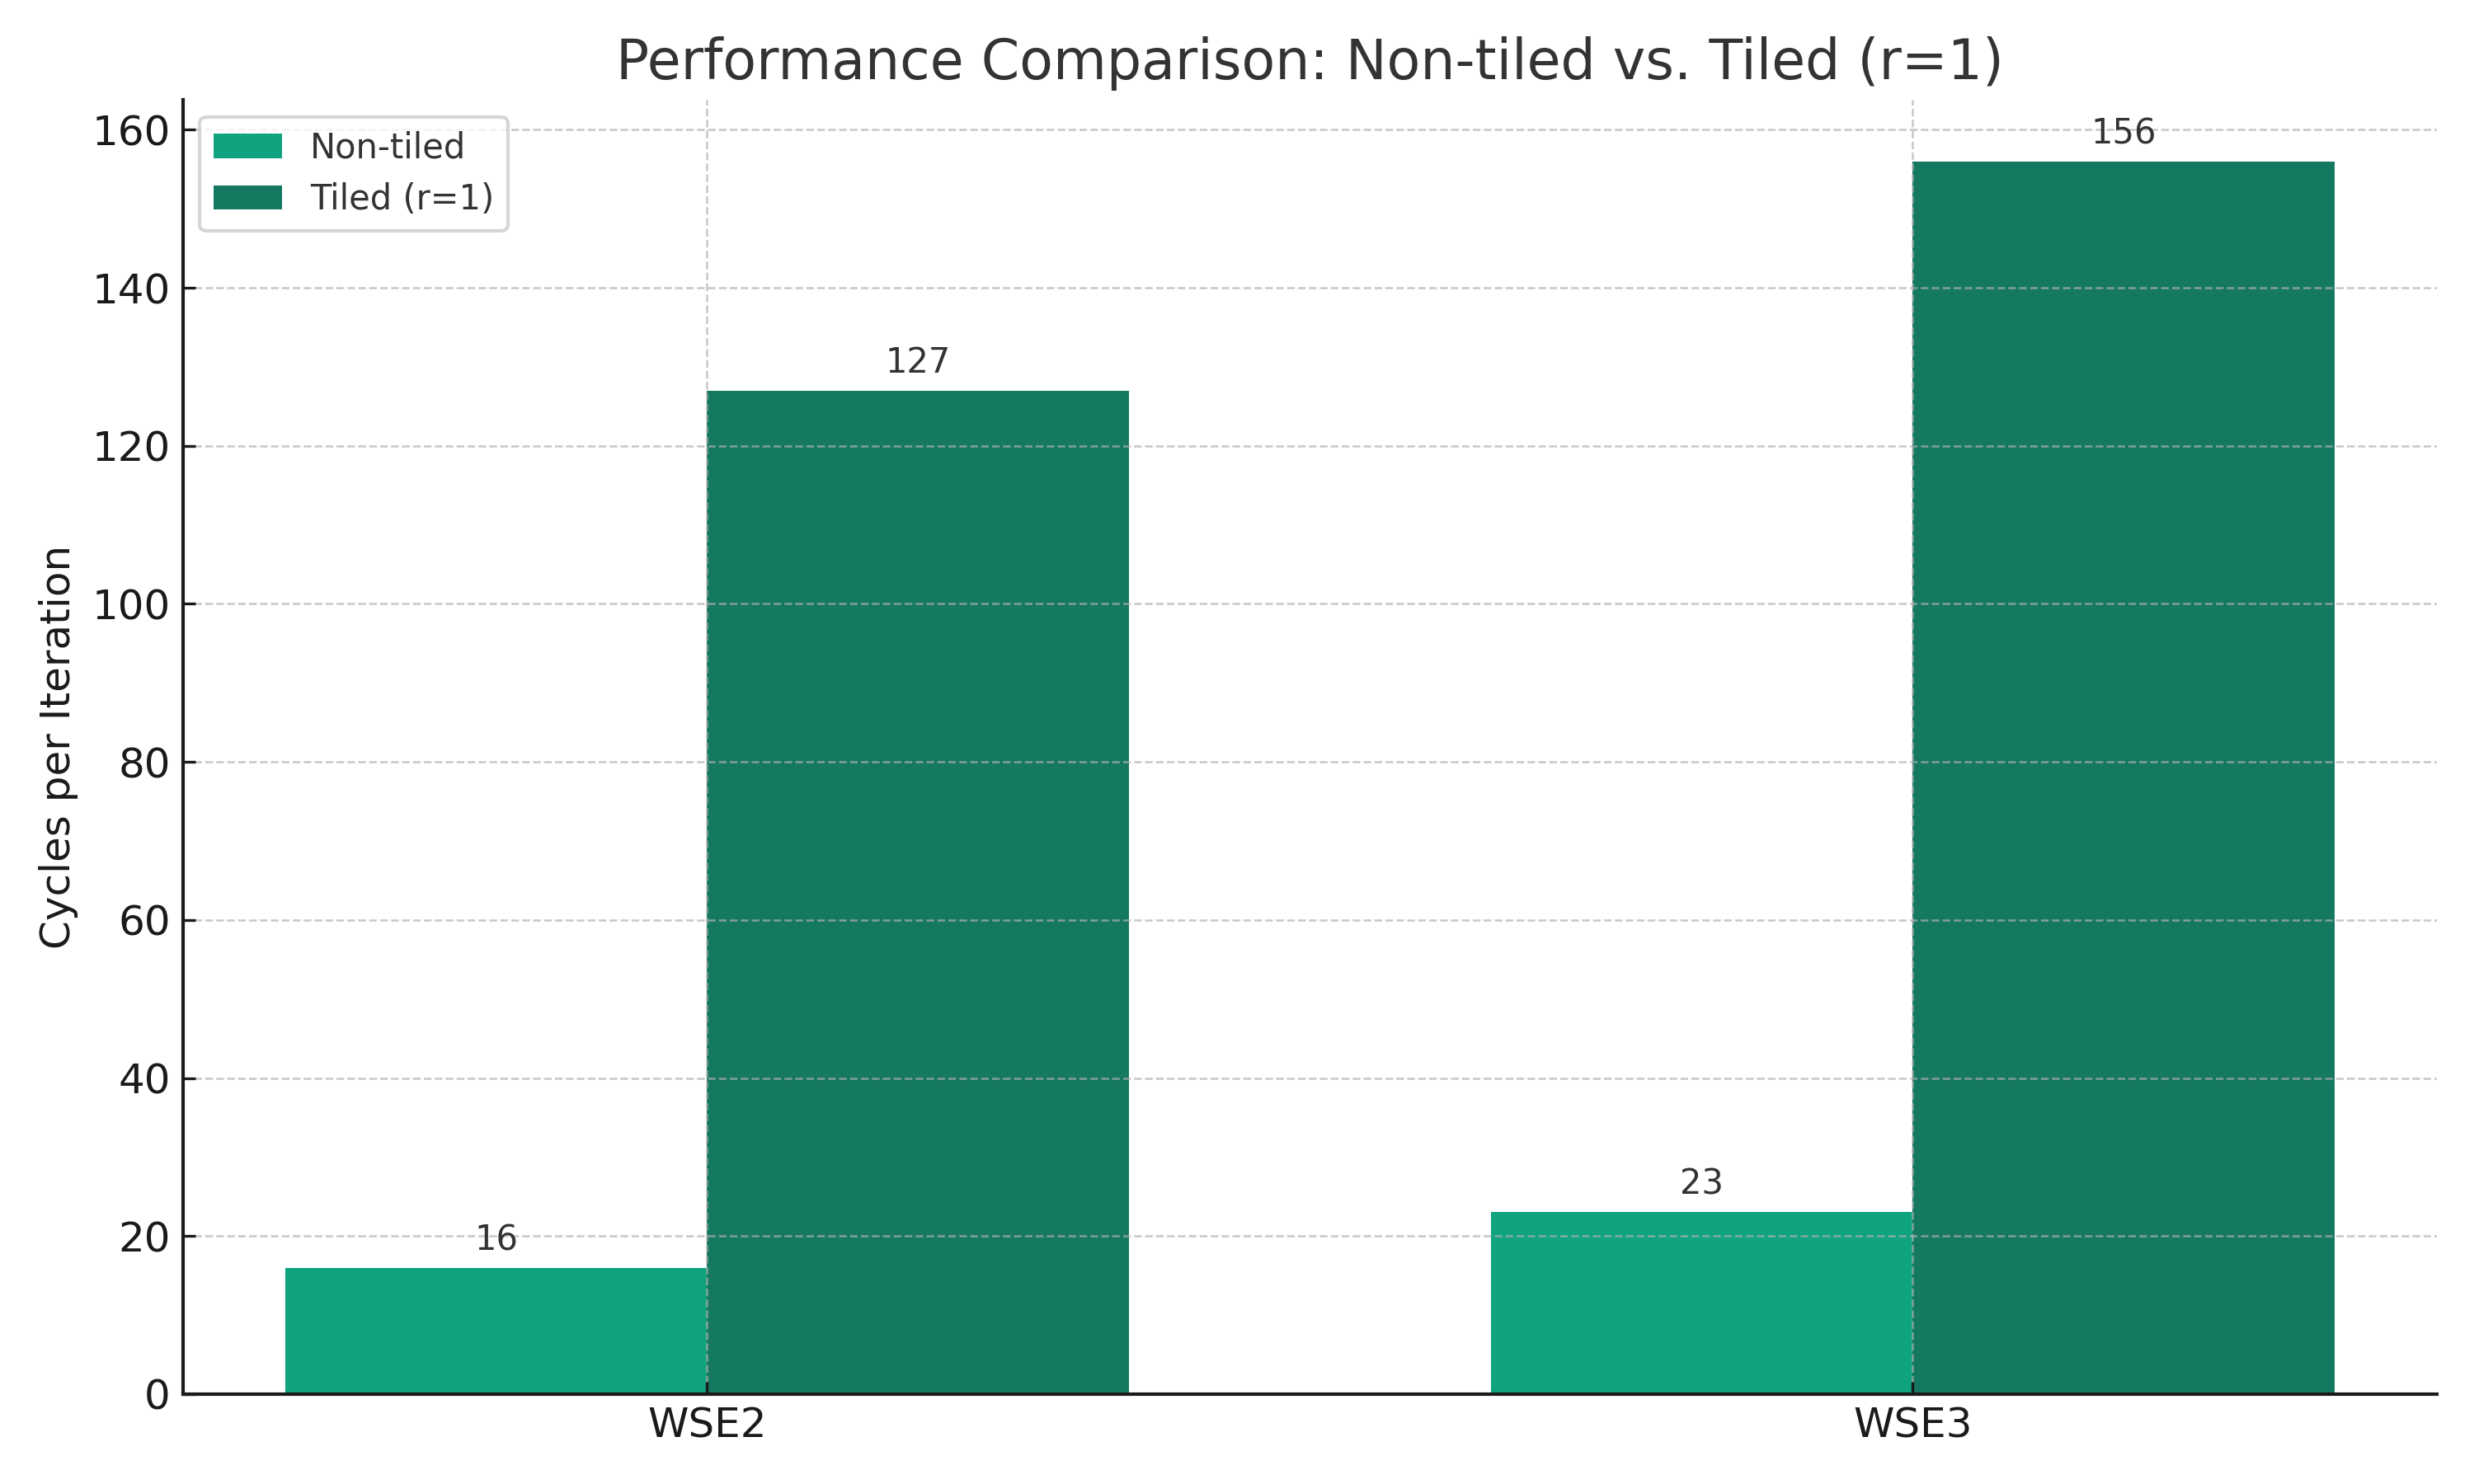
\includegraphics[width=0.5\linewidth]{plots/algo_comparison.png}
    \caption{Comparison of non-tiled and tiled algorithm for radius 1.}
    \label{fig:algo_comparison}
\end{figure}


\subsection{Comparison of Cerebras and traditional HPC-Arcitectures}
We conducted several experiments to compare the performance of the implemented stencils on the Cerebras WSE with highly optimized Devito implementations on CPU and GPU. The experiments were conducted in Vast.ai cloud.
As a CPU we used AMD EPYC 9554 64-Core Processor.
As a GPU we used NVIDIA H100 SXM 80GB.

For the first experiment, we ran the optimized stencil code on CPU and GPU and kept the product of grid size and number of iterations constant. This results in a constant number of total flops. 

\begin{figure}[h]
    \centering
    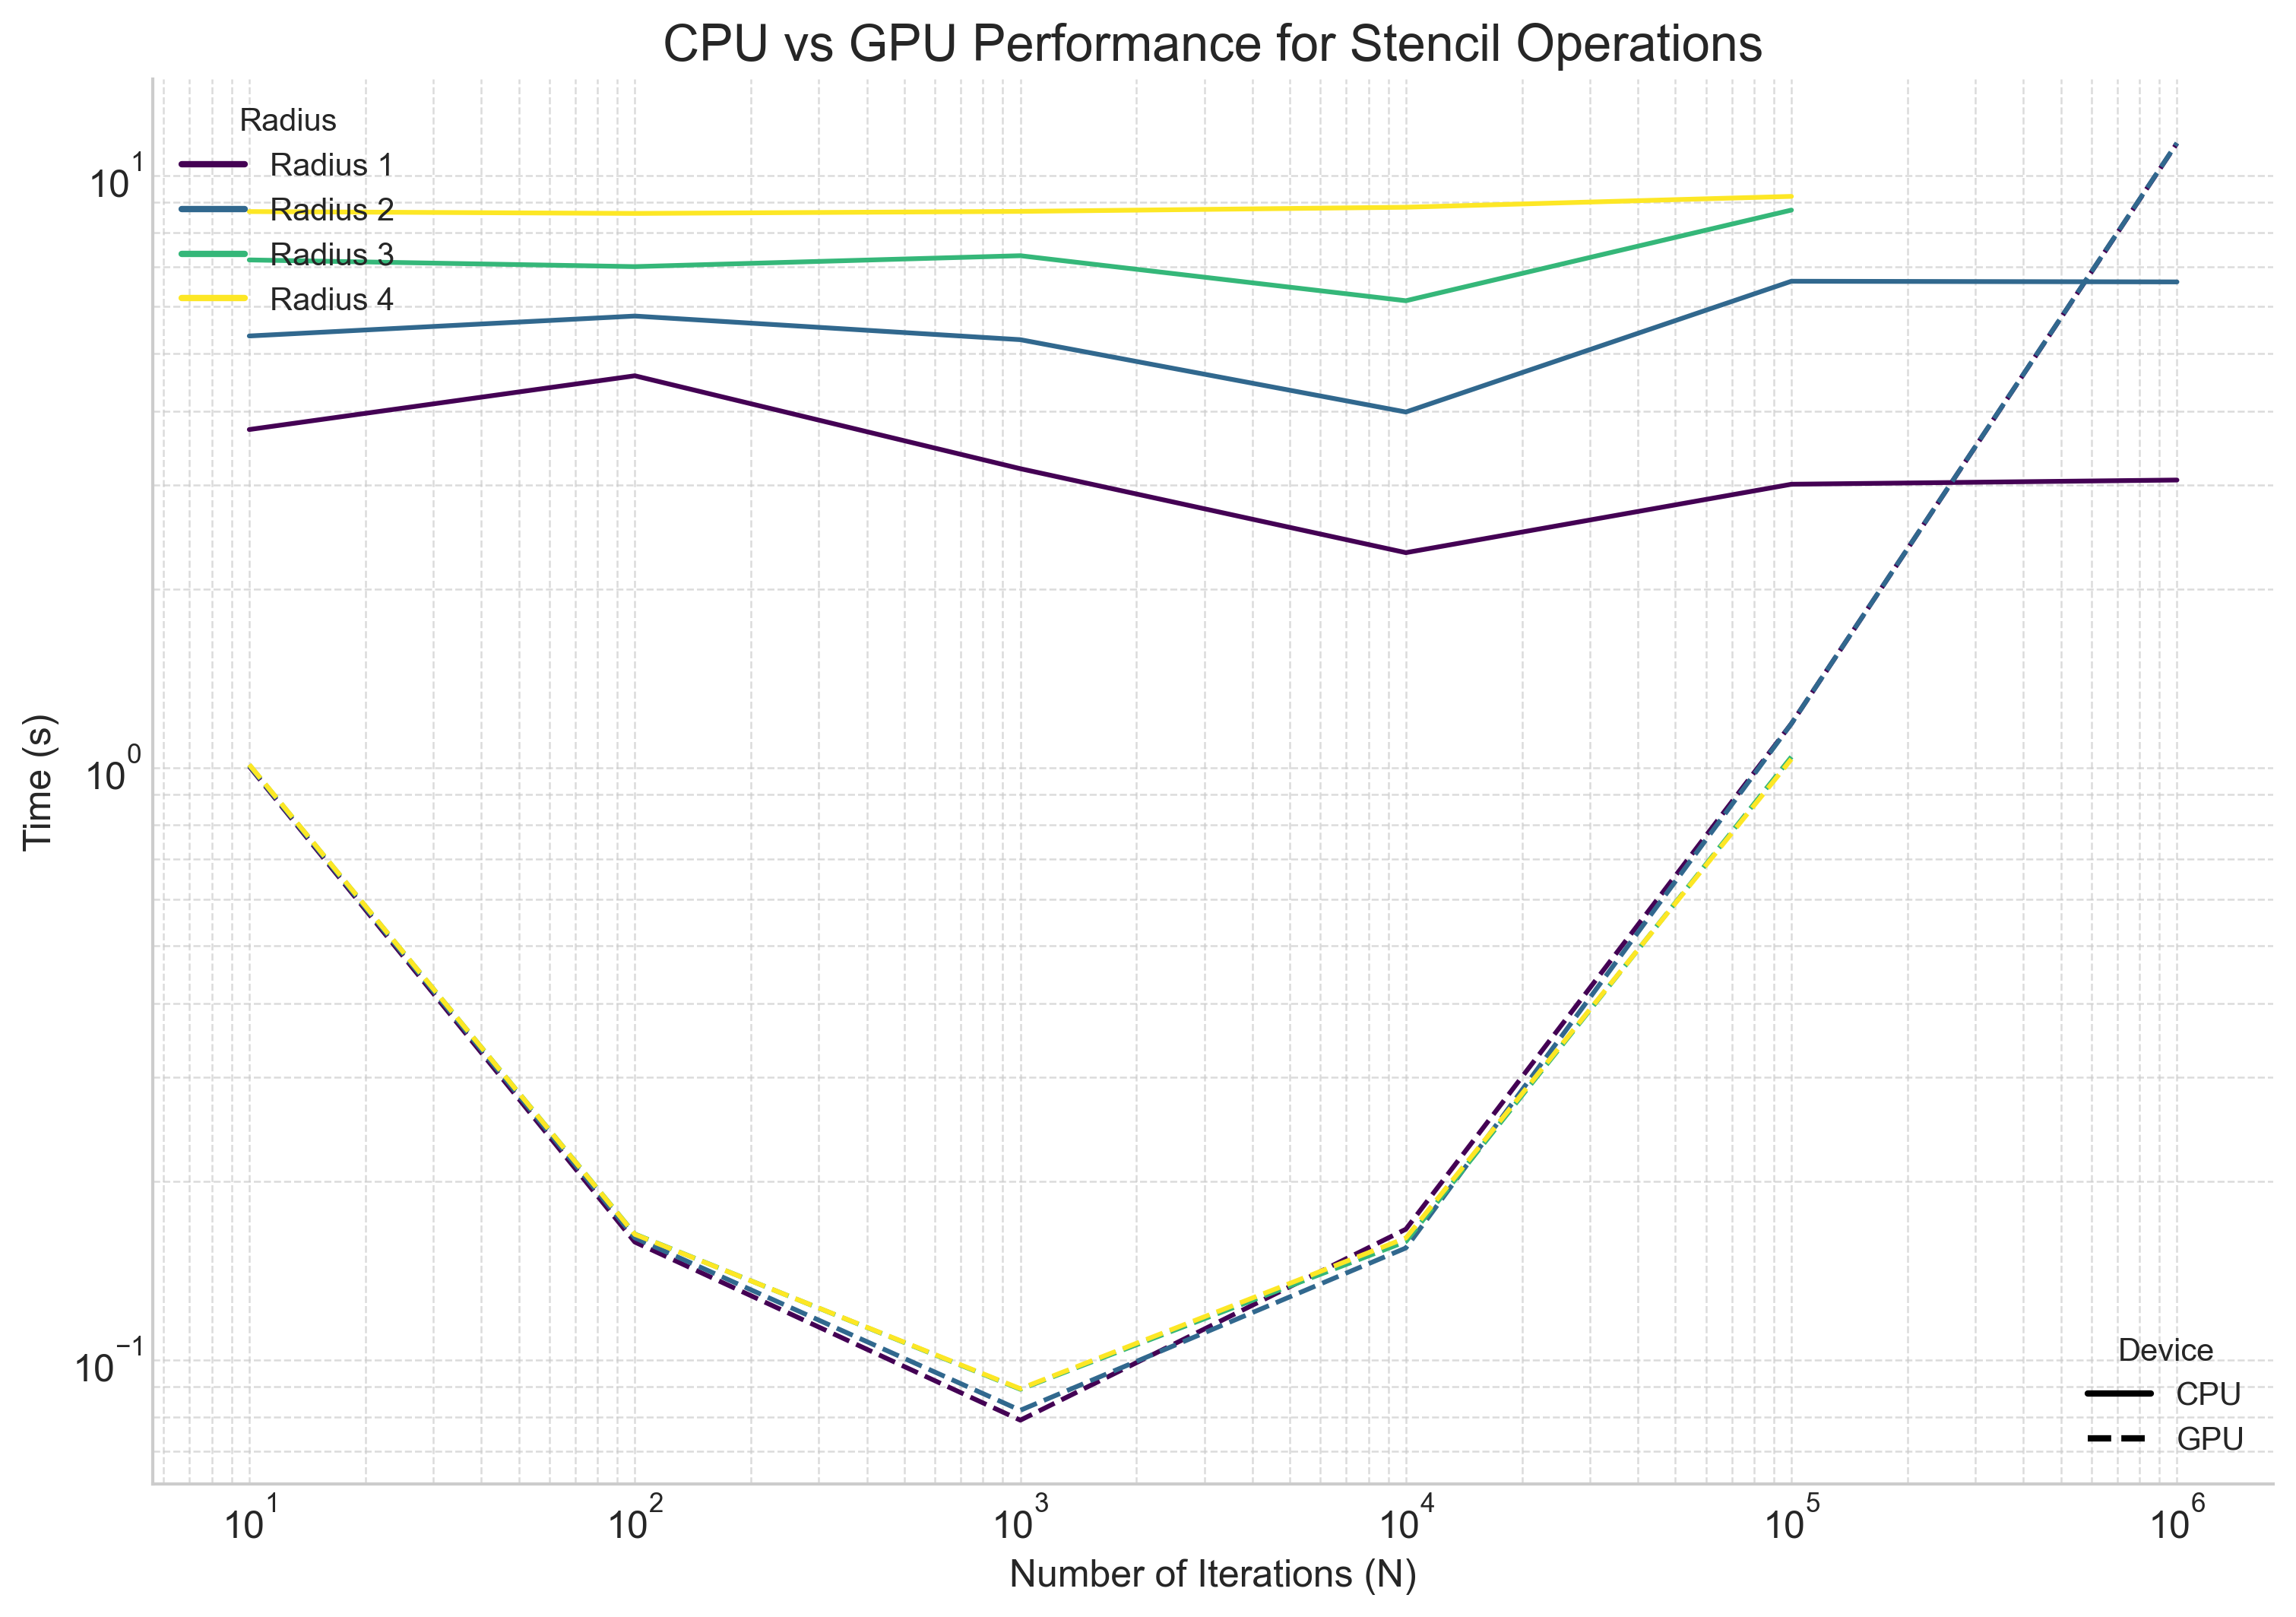
\includegraphics[width=0.5\linewidth]{plots/gpu_cpu_constant_product.png}
    \caption{Comparison of CPU and GPU performance for different grid sizes and number of iterations, so that $width \times height \times iterations = 10^10$.}
    \label{fig:gpu_cpu_constant_product}
\end{figure}

The results show that for most tested configurations, the gpu outperforms the cpu.
However for very small tile sizes of 100x100 and large iteration counts of $10^6$, the cpu is faster.

Furthermore we observe that GPU performance differs significantly depending on the racio between grid size and iterations with an optimal performance at $10^3$ iterations and a grid size of $10^7$. At this grid size, the data ($10^7$ numbers \times 4 bytes per number $=40MB$) fits perfectly into 50MB L2 cache of the H100. 

Notably the GPU perfors up to 100x worse for non-ideal grid sizes with $10^4$ elements compared to the ideal grid size with $10^7$ elements.

For CPU, the performance is not as sensitive to the ratio between grid size and iterations with just 2x worse performance for the least ideal grid size of $10^8$ elements compared to the ideal grid size of $10^6$ elements.

Another notable observation is that the cpu is a lot more sensitive to different radii (which do change the number of flops) than the gpu. For the cpu and its optimal grid size of $10^6$, it takes 3.8 times longer to calculate the 4 times as computationally expensive stencil with radius 4 compared to the stencil with radius 1. For the GPU on the other hand, it takes only 1.1 times as long for its optimal grid size of $10^7$.
This indicates that in their optimal configuration, the cpu is compute limited while the gpu is memory limited.

As a second experiment, we compared our implementation for a grid size of $10^7$ to the optimized gpu and cpu implementation. To fit a size of $10^3\times10^4$ on the WSE-2 with dimensions of $750\times994$, we need a tile size of at least $2x11$ and on WSE-3 with dimensions of $750\times1200$ a tile size of at least $14x1$. As shown in the earlier experiments, degrade larger tile sizes always the performance so we used these minimum tile sizes.




% Extrapolating the cerebras simulation results to this grid size, we find that the Cerebras implementation is about 100x faster on wse-2 and 140x faster on wse-3 than the GPU implementation. (calculate correct number here!!!)
for larger radii, we need to increase the shorter dimension of the tile.



h100 1e3 x 1e4 grid size, r=1: 0.0000791 s/iter -> 12.600 iter/s





This speedup gets even greater for the less ideal grid sizes for gpu.

Comparing the GPU implementation with our non-tiled algorithm using the largest possible grid size (WSE dimensions), we find that the Cerebras implementation is about 800x faster than the GPU implementation. (calculate correct number here!!!)

\subsection{Comparison of r1-optimized and non-optimized tiled algorithm}
We find that the r1-optimized tiled algorithm is significantly faster than the non-optimized tiled algorithm.
The difference can be seen in more detail in the next experiment.

\subsection{What contributes to the cycle count?}
We analyze the the instruction traces the simulator can record for what contributes to the the measured cycle counts.
We find that the effective simd width for some instructions in our implementation is lower than the theoretical maximum.
For \texttt{@fadds} it is 1.25 on wse-2 and 1.5 on wse-3.
The \texttt{@fmuls} instruction only have a simd width of 1 and we find that we measure exactly one cycle per instruction.

Here is a table that lists the different number of cycles per program segment.


\section{Discussion}
- why not full simd width?
- answer research questions from introduction
- why is wse3 slower than wse2?

\section{Future work???}
\begin{itemize}
    \item More optimization: use border PEs in a smarter way, use explicit dsr assignment,try to overlap communication and computation in the general algorithm, try achieving full simd width
    \item JOR, Gauss-Seidel / Red-Black implentation and SOR method or multigrid methods
    \item automatic convergence detection
\end{itemize}

\section{Bibliography}

\end{document}
